\chapter{Jet mass measurement in dijet and trijet final states}\label{chap:planner}
\section{Data and MC Samples}
\subsection{Data}\label{data}
The full Ultralegacy Run II datasets are used in this analysis. This data was taken in pp collisions in 2016, 2017, and 2018 at $\sqrt{s}=13$TeV (25 ns bunch crossings), corresponding to an integrated luminosity of 138 $\text{pb}^{-1}$. Due to differences in data-taking conditions, the dataset is split into 4 eras: 2016APV, 2016, 2017, and 2018 and correspond to integration luminosities of 19.50 $\text{pb}^{-1}$, 16.81 $\text{pb}^-1$, 41.48 $\text{pb}^{-1}$, and 59.83 $\text{pb}^{-1}$ respectively. The 2016 data is split into 2 separate datasets due to an issue in the analog pipeline voltage (APV) readout chips of the silicon strip tracker at the beginning of running in 2016. After the inefficiencies caused by this were discovered, an increase in the preamplifier feedback voltage bias (VFP) was able to recover the hit efficiency of the tracker to normal levels; however the data taken before this fix (2016APV) was already affected and mitigation of the effects was applied in offline reconstruction for it but not for those after the VFP increase (2016). \\
The data samples used and their names and eras are listed in Table \ref{table:1}. \\
Official Golden JSONs are employed to consider only the luminosity sections passing data-quality certification requirements.
\begin{itemize}
\item 2016 Data: \texttt{Cert\_271036-284044\_13TeV\_Legacy2016\_Collisions16\_JSON.txt}
\item 2017 Data: \texttt{Cert\_294927-306462\_13TeV\_UL2017\_Collisions17\_GoldenJSON.txt}
\item 2018 Data: \texttt{Cert\_314472-325175\_13TeV\_Legacy2018\_Collisions18\_JSON.txt}
\end{itemize}
% \usepackage{graphicx}
\begin{table}[h!]
	\centering
	\resizebox{\textwidth}{!}{%
		\begin{tabular}{ll}
			\hline
			Era & DAS dataset name \\ \hline
			UL2016APV B-ver1 & \texttt{/JetHT/Run2016B-ver1\_HIPM\_UL2016\_MiniAODv2\_NanoAODv9-v2/NANOAOD} \\
			UL2016APV B-ver2 & \texttt{/JetHT/Run2016B-ver2\_HIPM\_UL2016\_MiniAODv2\_NanoAODv9-v2/NANOAOD} \\
			UL2016APV C & \texttt{/JetHT/Run2016C-HIPM\_UL2016\_MiniAODv2\_NanoAODv9-v2/NANOAOD} \\
			UL2016APV D & \texttt{/JetHT/Run2016D-HIPM\_UL2016\_MiniAODv2\_NanoAODv9-v2/NANOAOD} \\
			UL2016APV E & \texttt{/JetHT/Run2016E-HIPM\_UL2016\_MiniAODv2\_NanoAODv9-v2/NANOAOD} \\
			UL2016APV F & \texttt{/JetHT/Run2016F-HIPM\_UL2016\_MiniAODv2\_NanoAODv9-v2/NANOAOD} \\ \hline
			UL2016 F & \texttt{/JetHT/Run2016F-UL2016\_MiniAODv2\_NanoAODv9-v1/NANOAOD} \\
			UL2016 G & \texttt{/JetHT/Run2016G-UL2016\_MiniAODv2\_NanoAODv9-v1/NANOAOD} \\
			UL2016 H & \texttt{/JetHT/Run2016H-UL2016\_MiniAODv2\_NanoAODv9-v1/NANOAOD} \\ \hline
			UL2017 B & \texttt{/JetHT/Run2017B-UL2017\_MiniAODv2\_NanoAODv9-v1/NANOAOD} \\
			UL2017 C & \texttt{/JetHT/Run2017C-UL2017\_MiniAODv2\_NanoAODv9-v1/NANOAOD} \\
			UL2017 D & \texttt{/JetHT/Run2017D-UL2017\_MiniAODv2\_NanoAODv9-v1/NANOAOD} \\
			UL2017 E & \texttt{/JetHT/Run2017E-UL2017\_MiniAODv2\_NanoAODv9-v1/NANOAOD} \\
			UL2017 F & \texttt{/JetHT/Run2017F-UL2017\_MiniAODv2\_NanoAODv9-v1/NANOAOD} \\ \hline
			UL2018 A & \texttt{/JetHT/Run2018A-UL2018\_MiniAODv2\_NanoAODv9-v2/NANOAOD} \\
			UL2018 B & \texttt{/JetHT/Run2018B-UL2018\_MiniAODv2\_NanoAODv9-v1/NANOAOD} \\
			UL2018 C & \texttt{/JetHT/Run2018C-UL2018\_MiniAODv2\_NanoAODv9-v1/NANOAOD} \\
			UL2018 D & \texttt{/JetHT/Run2018D-UL2018\_MiniAODv2\_NanoAODv9-v2/NANOAOD} \\ \hline
		\end{tabular}%
	}\caption{Full Run 2 Ultra Legacy datasets used in this analysis. }
\label{table:1}
\end{table}
\subsection{Monte Carlo Simulation}\label{MC}
The simulation of the pp collision events is performed using various Monte Carlo (MC) software packages in multiple steps. The matrix-element generation for the samples used in the analyses is handled by MADGRAPH5 aMC@NLO v2.6.5 (v2.6.1) \cite{madgraph}. The samples are then interfaced with PYTHIA 8.244 \cite{pythia8} for parton showering and hadronization. All samples used in this dataset and their cross-sections are show in Table \ref{table:2}.\\
All samples were generated using PYTHIA8 settings; in them the CP5 tune \cite{CP5} is used and NNPDF3.1 \cite{nnpdf} PDF sets for the modeling of the parton distribution functions are used. The generated events are then passed through the GEANT4 \cite{geant4} package to simulate the detector response before they are treated with the same reconstruction algorithms as the real data. As a cross-check and for calculation of the parton shape and scale uncertainties, additional samples of MADGRAPH interfaced with HERWIG7 \cite{herwig}  with tune CH3 are used. These samples are shown in Table \ref{table:3}.\\
% TODO -- what are the exact versions of madgraph and pythia used in these MC samples and is it NNNPDF3.1 used?
\begin{table}[h!]
	\centering
	\resizebox{\textwidth}{!}{%
		\begin{tabular}{ll}
			\hline
			DAS Dataset & XS \\ \hline
			\texttt{QCD\_HT200to300\_TuneCP5\_PSWeights\_13TeV-madgraphMLM-pythia8} & 1554000.0 \\
			\texttt{QCD\_HT300to500\_TuneCP5\_PSWeights\_13TeV-madgraphMLM-pythia8} & 323800.0  \\
			\texttt{QCD\_HT500to700\_TuneCP5\_PSWeights\_13TeV-madgraphMLM-pythia8} & 30280.0 \\
			\texttt{QCD\_HT700to1000\_TuneCP5\_PSWeights\_13TeV-madgraphMLM-pythia8} & 6392.0 \\
			\texttt{QCD\_HT1000to1500\_TuneCP5\_PSWeights\_13TeV-madgraphMLM-pythia8} & 1118.0 \\
			\texttt{QCD\_HT1500to2000\_TuneCP5\_PSWeights\_13TeV-madgraphMLM-pythia8} & 108.9 \\
			\texttt{QCD\_HT2000toInf\_TuneCP5\_PSWeights\_13TeV-madgraphMLM-pythia8} & 21.93  \\ \hline
		\end{tabular}%
	}\caption{Madgraph MLM + Pythia8 datasets and cross sections.
}\label{table:2}
\end{table}
\begin{table}[h!]
	\centering
	\resizebox{\textwidth}{!}{%
		\begin{tabular}{ll}
			\hline
			DAS Dataset & XS \\ \hline
			\texttt{QCD\_HT200to300\_TuneCH3\_13TeV-madgraphMLM-herwig7} & 883.5 \\
			\texttt{QCD\_HT300to500\_TuneCH3\_13TeV-madgraphMLM-herwig7} & 259.6  \\
			\texttt{QCD\_HT500to700\_TuneCH3\_13TeV-madgraphMLM-herwig7} & 23.63 \\
			\texttt{QCD\_HT700to1000\_TuneCH3\_13TeV-madgraphMLM-herwig7} & 4.943 \\
			\texttt{QCD\_HT1000to1500\_TuneCH3\_13TeV-madgraphMLM-herwig7} & 0.8013  \\
			\texttt{QCD\_HT1500to2000\_TuneCH3\_13TeV-madgraphMLM-herwig7} & 0.06815\\
			\texttt{QCD\_HT2000toInf\_TuneCH3\_13TeV-madgraphMLM-herwig7} & 0.01245 \\ \hline
		\end{tabular}%
	}\caption{Madgraph MLM + HERWIG7 and cross sections.}\label{table:3}
\end{table}
\section{Event Selection}
This section describes how events are selected at the trigger and particle level.
\subsection{Trigger Selection}
% TODO: add more information about how triggers fire
The data used for the dijet and trijet analyses are collected using single jet triggers at the High Level Trigger (HLT) that trigger based on the jet's transverse momentum. The L1 and HLT thresholds for each of the triggers are listed in table \ref{table:tab1}. As done in Ref. \cite{1605_IncJet}, we divide the events into independent regions as a function of leading jet \pt. In each region only one trigger is used and there is no overlap between regions to avoid double counting. The regions are chosen so that each trigger assigned to it is fully efficient. The edges of the trigger regions are then also used as the \pt bin edges for the jet cross sections so no \pt bin has more than one trigger.\\
The trigger efficiencies are calculated using the emulator method, where the trigger decision is emulated in data using the trigger objects of a reference trigger, trig\textsubscript{ref}. To reproduce the trigger decision, objects from both trigger levels are needed, L1 and HLT. Under the assumption that the reference trigger is fully efficient for the considered phase space of the desired trigger, the efficiency is defined as:
\begin{equation}\label{eq:1}
\epsilon_{{\rm trig_i}}=\frac{\rm Events\left({\rm L1Object}\_\pt>\pt_{{\rm ref}}\quad \& \quad {\rm HLTObject\_\pt>\pt_i \quad\&\quad trig_{ref}} \right)} { \rm Events \left( trig_{ref} \right) }
\end{equation}
where trig\textsubscript{i} is the trigger of interest. For example, if we wanted to calculate the effciency of the HLTPFJetAK8\_200 trigger, we would find the number of events that passed the reference trigger, HLTPFJetAK8\_140, have an L1 seed \pt greater than the reference trigger's, L1Object\_\pt\textgreater140, and an HLT object \pt greater than the trigger in question, HLTObject\_\pt\textgreater200. Then divide this by the total number of events that pass trig\textsubscript{ref}. The complete list of triggers with their reference triggers and L1 and HLT threshold \pt's are shown in Table \ref{table:tab1}.\\
\begin{table}[h!]
  \centering
	\resizebox{\textwidth}{!}{%
		\begin{tabular}{@{}llllllll@{}}
			\hline
			Trigger & Reference Trigger & \begin{tabular}[c]{@{}l@{}} L1 Threshold\\ (GeV) \end{tabular} & \begin{tabular}[h!]{@{}l@{}} HLT Threshold \\ (GeV)\end{tabular} & \begin{tabular}[c]{@{}l@{}}Full efficiency \\ threshold 2016 \\ (GeV)\end{tabular} & \begin{tabular}[c]{@{}l@{}}Full efficiency \\ threshold 2016APV \\ (GeV)\end{tabular} & \begin{tabular}[c]{@{}l@{}}Full efficiency \\ threshold 2017 \\ (GeV)\end{tabular} & \begin{tabular}[c]{@{}l@{}}Full efficiency\\ threshold 2018 \\ (GeV)\end{tabular} \\ \hline
			HLT\_AK8PFJet60 & HLT\_AK8PFJet40 & 0 & 60 & 178 & 0 & 0 & 0 \\
			HLT\_AK8PFJet80 & HLT\_AK8PFJet60 & 60 & 80 & 205 & 181 & 168 & 177 \\
			HLT\_AK8PFJet140 & HLT\_AK8PFJet80 & 80 & 140 & 295 & 295 & 267 & 281 \\
			HLT\_AK8PFJet200 & HLT\_AK8PFJet140 & 140 & 200 & 379 & 389 & 359 & 394 \\
			HLT\_AK8PFJet260 & HLT\_AK8PFJet200 & 200 & 260 & 459 & 463 & 447 & 484 \\
			HLT\_AK8PFJet320 & HLT\_AK8PFJet260 & 260 & 320 & 544  & 554 & 537 & 570 \\
			HLT\_AK8PFJet400 & HLT\_AK8PFJet360 & 320 & 400 & 643 & 664 & 646 & 683 \\
			HLT\_AK8PFJet450 & HLT\_AK8PFJet440 & 400 & 450 & 702 & 733 & 718 & 751 \\
			HLT\_AK8PFJet500 & HLT\_AK8PFJet530 & 450 & 500 & 802 & 838 & 791 & 817 \\
			HLT\_AK8PFJet550 & HLT\_AK8PFJet630 & 500 & 550 & N/A & N/A & 887 & 884 \\ \hline
		\end{tabular}
		%
	}
\caption{List of available triggers for our \pt range with corresponding reference triggers, and their \pt thresholds at L1 and HLT. The \pt threshold corresponding to the starting point of full efficiency is also specified for each trigger and year.}
\label{table:tab1}
\end{table}
Each trigger has a turn-on curve, and the \pt at which these curves plateau, and the trigger becomes fully efficient ($>$ 0.99), can be derived from a fit using the following equation:
\begin{equation} \label{eq:2}
%\epsilon = 0.5*\left(1+\textrm{erf}\left(\frac{x-b}{\sqrt{2}c} \right)\right)
%  \epsilon = a+0.5(1-a)\left(1+\textrm{erf}\left(\frac{x-b}{c} \right)\right)
  \epsilon = a\left(b+\frac{1-b}{2}\left(1-\text{erf}\left(\frac{x-c}{d}\right)\right)\right)
\end{equation}
where b and c are free parameters. Figure \ref{fig:4} shows the results of this fit to the efficiency as a function of \pt for trigger HLTPFJetAK8\_200 trigger, and the threshold \pt, which is found by inverting Eq. \ref{eq:1} and setting it equal to 0.99. The plots for the rest of the available triggers can be found in the Appendix.
\begin{equation}
\pt  =c+d*\text{erf}^{-1}(1-((0.99/a - b)/(0.5*(1-b))))
\end{equation}
The resulting turn-on \pt's are used to assign the correct trigger and corresponding prescale to that event. Continuing our previous example, if a 2016 event has passed the HLTPFJetAK8\_200 trigger, and has a leading jet \pt between 459 GeV and 544 GeV (see tab. \ref{table:tab1}, that event will be assigned the trigger HLTPFJetAK8\_200 and its corresponding prescale.
\begin{figure}[h!]
	\centering
	\begin{subfigure}
		\centering
		\includegraphics[width=0.45\textwidth]{figures/multijet/2016APV_trig_eff/efficiency_HLT_AK8PFJet200.png}
	\end{subfigure}%
	\begin{subfigure}
		\centering
		\includegraphics[width=0.45\textwidth]{figures/multijet/2016_trigg_eff/efficiency_HLT_AK8PFJet200.png}
	\end{subfigure}
	\begin{subfigure}
		\centering
		\includegraphics[width=0.45\textwidth]{figures/multijet/2017_trig_eff/efficiency_HLT_AK8PFJet200.png}
	\end{subfigure}%
	\begin{subfigure}
		\centering
		\includegraphics[width=0.45\textwidth]{figures/multijet/2018_trig_eff/efficiency_HLT_AK8PFJet200.png}
	\end{subfigure}
	\caption{HLT\_AK8PFJet200 Trigger efficiencies for 2016APV (top left), 2016 (top right), 2017 (bottom left), and 2018 (bottom right).}
	\label{fig:4}
\end{figure}
The trigger prescale values vary from run to run and even from lumisection to lumisection. All of the trigger values are available in brilcalc TRG \cite{brilcalc}, and we use the event pt, run information, and lumisection to map it to the correct prescale value before applying it. The trigger path assignment and prescale application is illustrated in figure \ref{fig:trigstitch}. Once the correct prescale for each event has been found, it is stored as an event weight.
\begin{figure}[h!]
  \begin{subfigure}
	\centering
	\includegraphics[width=0.9\textwidth]{figures/multijet/2016APV_TrigPlots.png}
\end{subfigure}
\begin{subfigure}
	\centering
	\includegraphics[width=0.9\textwidth]{figures/multijet/2016_TrigPlots.png}
\end{subfigure}
\begin{subfigure}
	\centering
	\includegraphics[width=0.9\textwidth]{figures/multijet/2017_TrigPlots.png}
\end{subfigure}
\begin{subfigure}
	\centering
	\includegraphics[width=0.9\textwidth]{figures/multijet/2018_TrigPlots.png}
\end{subfigure}
	\caption{All trigger paths available for all events (left), all trigger paths with prescales applied (center), all events sorted by trigger path with prescales applied and doubled events removed (right) for 2016, 2016APV, 2017, and 2018}
	\label{fig:trigstitch}
      \end{figure}
The turn-on \pt's are also used to select the \pt binning for the final measurement. Since we are combining all of the data-taking eras into one final result, for simplicity we take an approximation of the largest turn-on \pt for each trigger for the final \pt binning of [200, 290, 400, 480, 570, 680, 760, 840, 890, $\inf$]. Since there are substantially fewer events in the 840 and 890 GeV bins, we combine them together with the $\inf$ bin for an initial \pt binning of  [200, 290, 400, 480, 570, 680, 760, 840, 890, $\inf$] that is further  optimized for unfolding in section \ref{unfolding}.
\subsection{Jet selection}\label{selection}
The events selected by the triggers described above are then used in the full selections for the dijet and trijet events. The dijet selection is based on previous analyses \cite{1605_IncJet}, \cite{dijetZjet2013} and prioritize a back-to-back topology, while the trijet selection  has been optimized to increase gluon selection based on Ref. \cite{pureSamples}. All jets used are AK8 jets reconstructed as described in section \ref{jets} and passing the tight jet id criteria \cite{jetid}. %describe tight jet criteria??
For the dijet events, we require:
\begin{itemize}
	\item At least two jets with \pt\textgreater\, 200 GeV and $y < 2.5$,
	\item $\Delta\phi < 2.0$ and $\pt_{assym}<0.3$ between the leading two jets,
\end{itemize}
and select the two leading jets within each event.
For the trijet events we require:
\begin{itemize}
	\item At least three jets with \pt\textgreater\, 200 GeV and $y < 2.5$,
	\item $\Delta\phi < 1.0$ between each of the leading three jets,
\end{itemize}
and select the third softest jet of each event, as this is the jet most likely to be gluon-initiated.
% Describe jet veto maps
Figures \ref{fig:15} and \ref{fig:16} show the Data to MC agreement after selection. In these plots, the MG+Pythia8 distribution are scaled to the integral of the data. The considerable data to MC disagreement stems from the difficulty to model multijet QCD events in simulation. Figures \ref{fig:17} and \ref{fig:18} show the agreement between data and simulation for the ungroomed and groomed mass within each final \pt bin chosen for unfolding for dijet events, repsectively.  SImilarly, figures \ref{fig:19} and \ref{fig:20} show the agreement between data and simulation forthe ungroomed and groomed mass within each final \pt bin chosen for unfolding for the trijet events. Again, the simulation distributions are scaled to the integral of the data distirbution, but now normalised within each \pt bin.
\begin{figure}[h!]
  \centering
  \begin{subfigure}
    \centering
    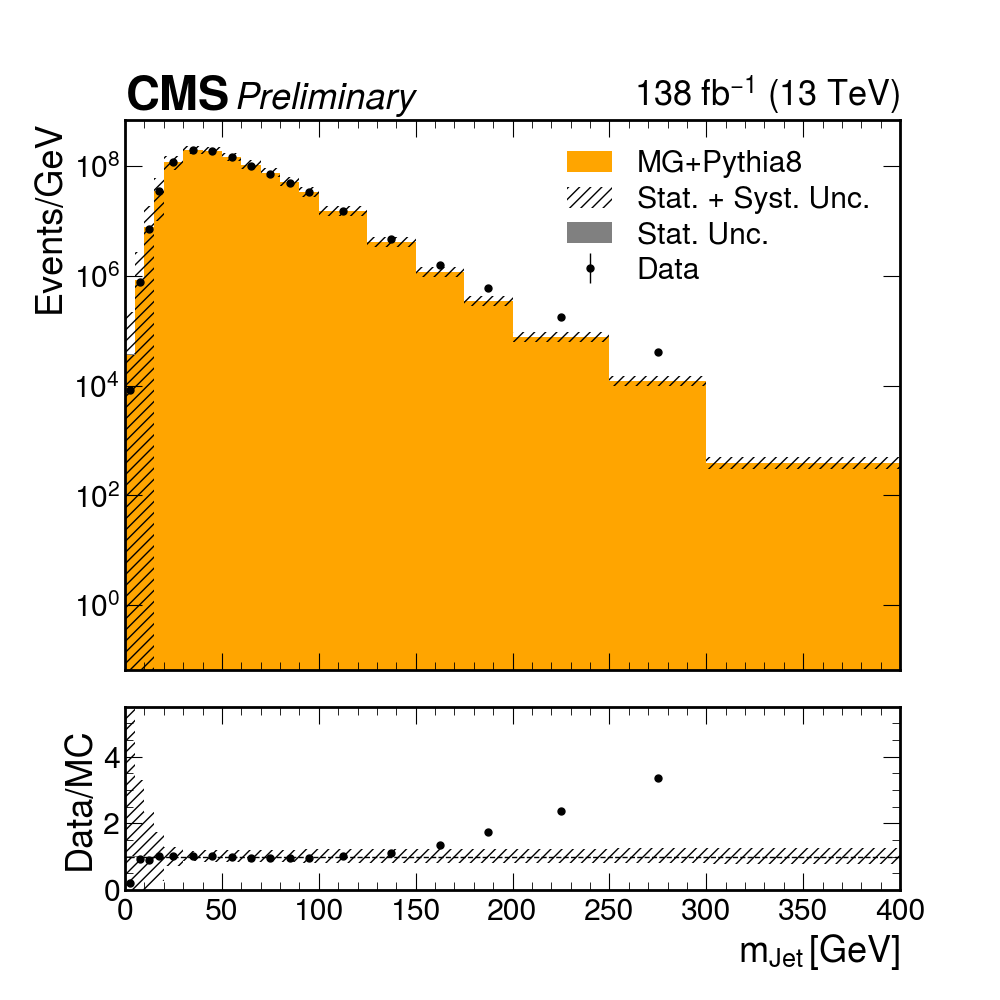
\includegraphics[width=0.45\textwidth]{figures/multijet/dijet/mjet_allyears_coarsebin.png}
  \end{subfigure}
  \begin{subfigure}
    \centering
    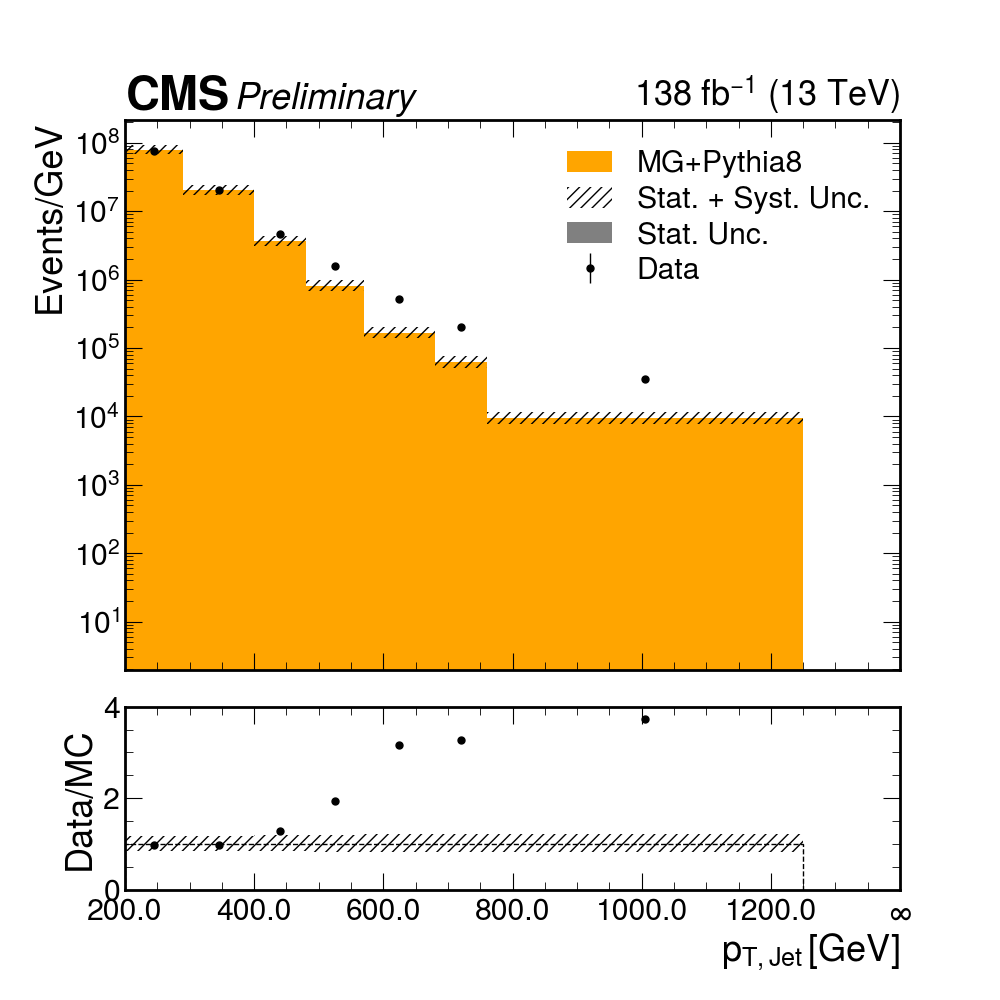
\includegraphics[width=0.45\textwidth]{figures/multijet/dijet/pt_allyears_coarsebin.png}
  \end{subfigure}
  \begin{subfigure}
    \centering
    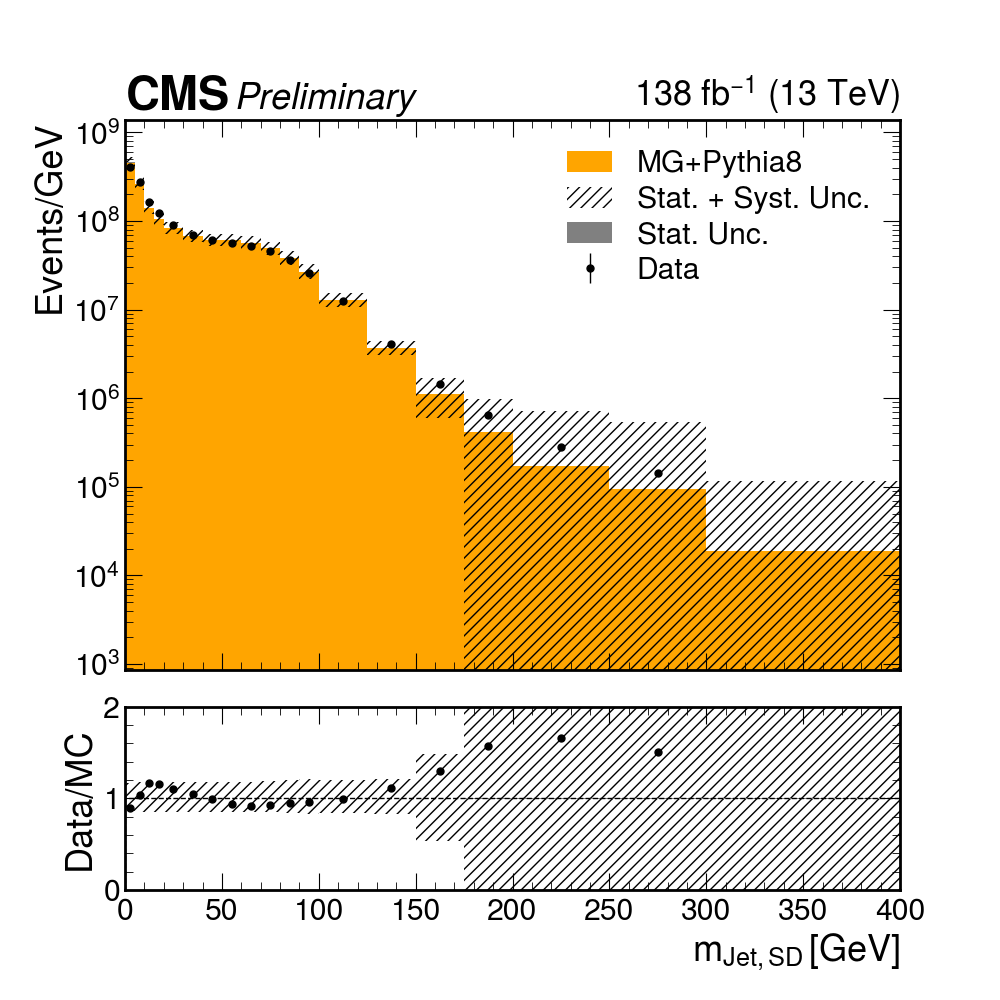
\includegraphics[width=0.45\textwidth]{figures/multijet/dijet/msd_allyears_coarsebin.png}
  \end{subfigure}
  \begin{subfigure}
    \centering
    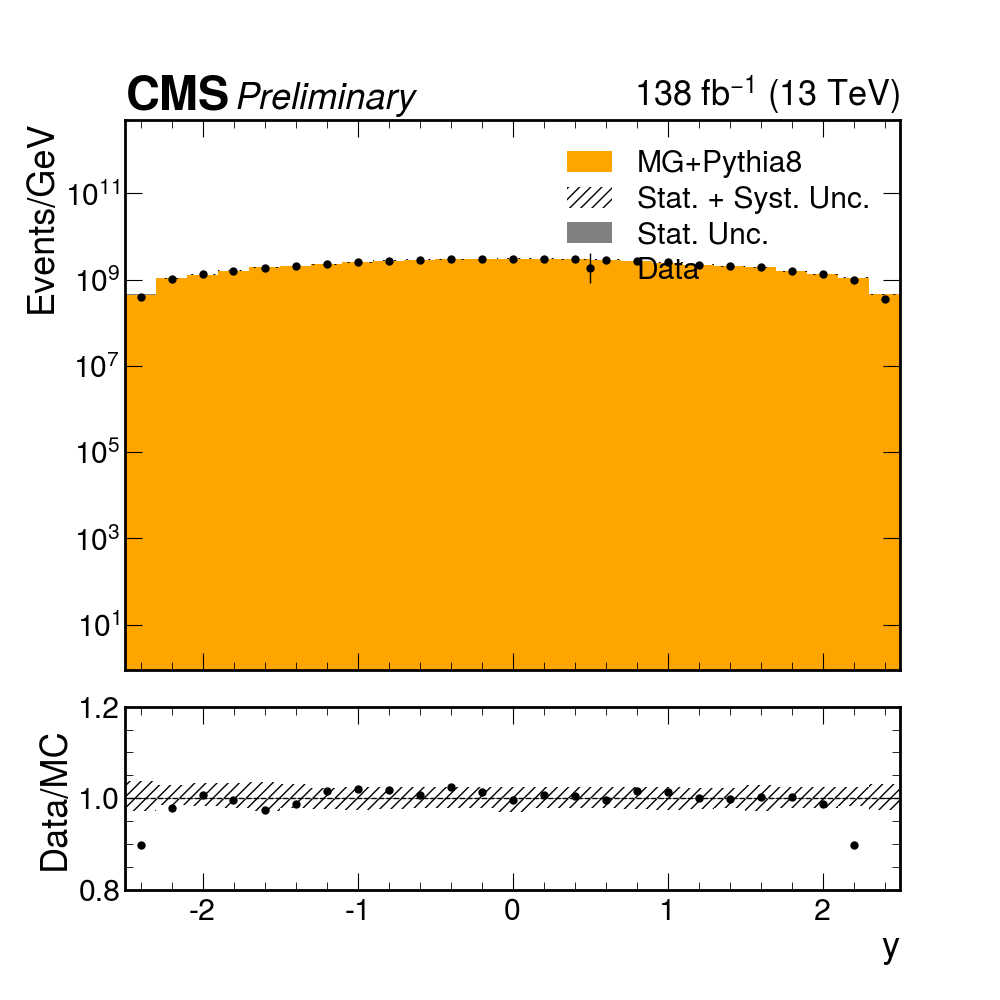
\includegraphics[width=0.45\textwidth]{figures/multijet/dijet/rap_allyears_coarsebin.png}
  \end{subfigure}
  \begin{subfigure}
    \centering
    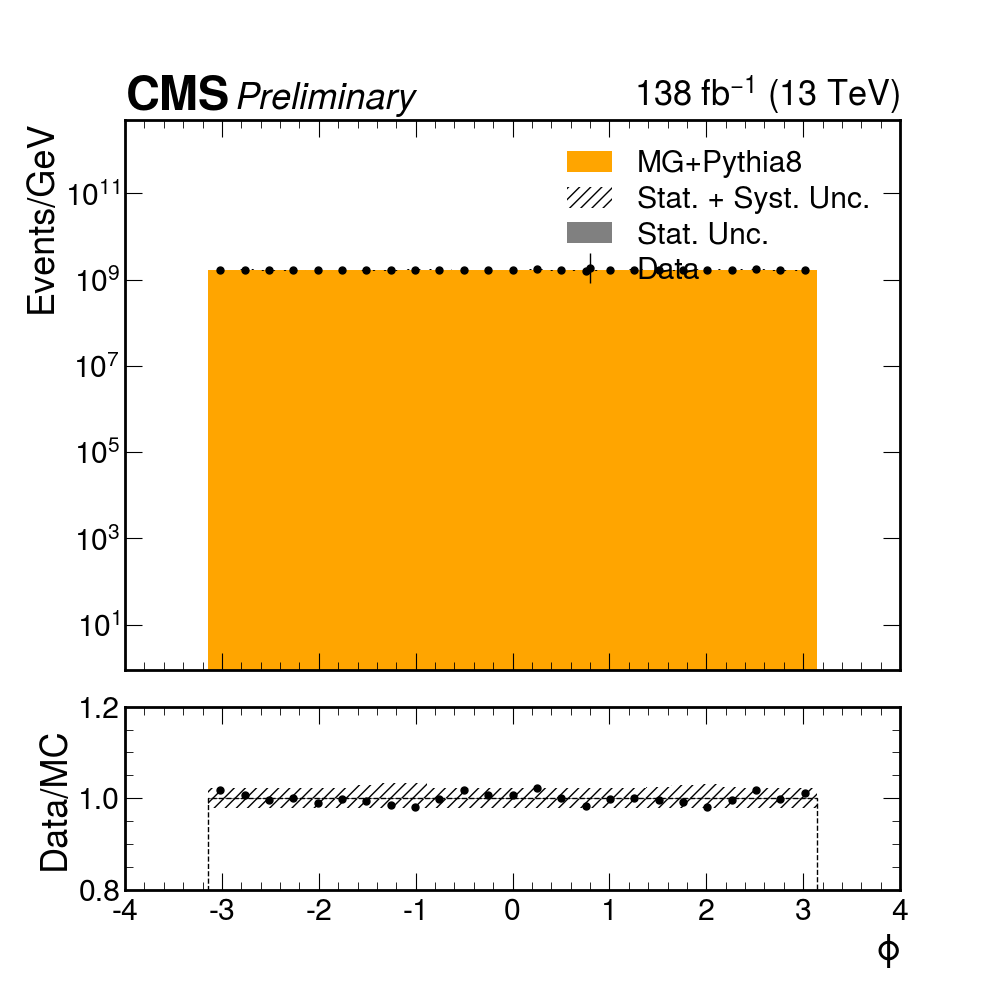
\includegraphics[width=0.45\textwidth]{figures/multijet/dijet/phi_allyears_coarsebin.png}
  \end{subfigure}
  \caption{Full Run 2 UL dijet Data to MC comparison for ungroomed mass (top left), transverse momentum (top right), softdrop mass (center left), rapidity (center right), and phi (bottom).}
	\label{fig:15}
\end{figure}
\begin{figure}[h!]
  \centering
  \begin{subfigure}
    \centering
    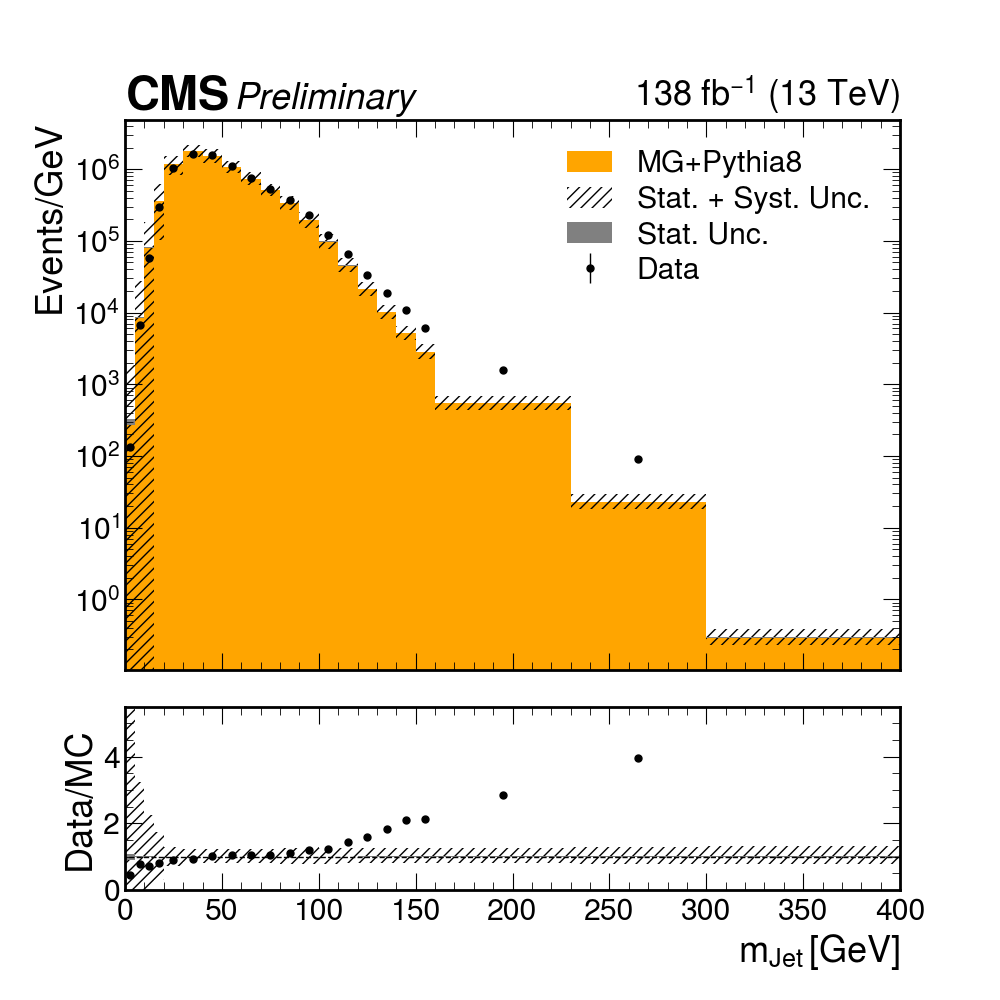
\includegraphics[width=0.45\textwidth]{figures/multijet/trijet/mjet_allyears_coarsebin.png}
  \end{subfigure}
  \begin{subfigure}
    \centering
    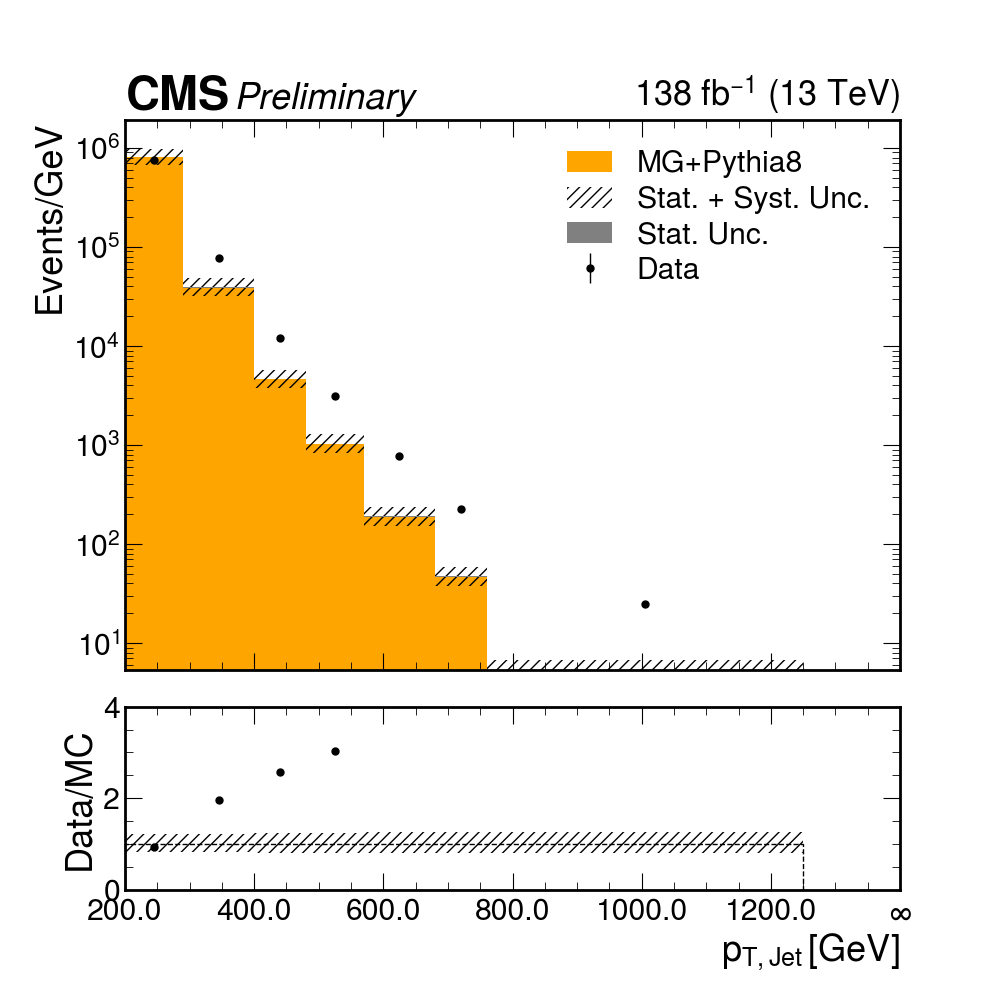
\includegraphics[width=0.45\textwidth]{figures/multijet/trijet/pt_allyears_coarsebin.png}
  \end{subfigure}
  \begin{subfigure}
    \centering
    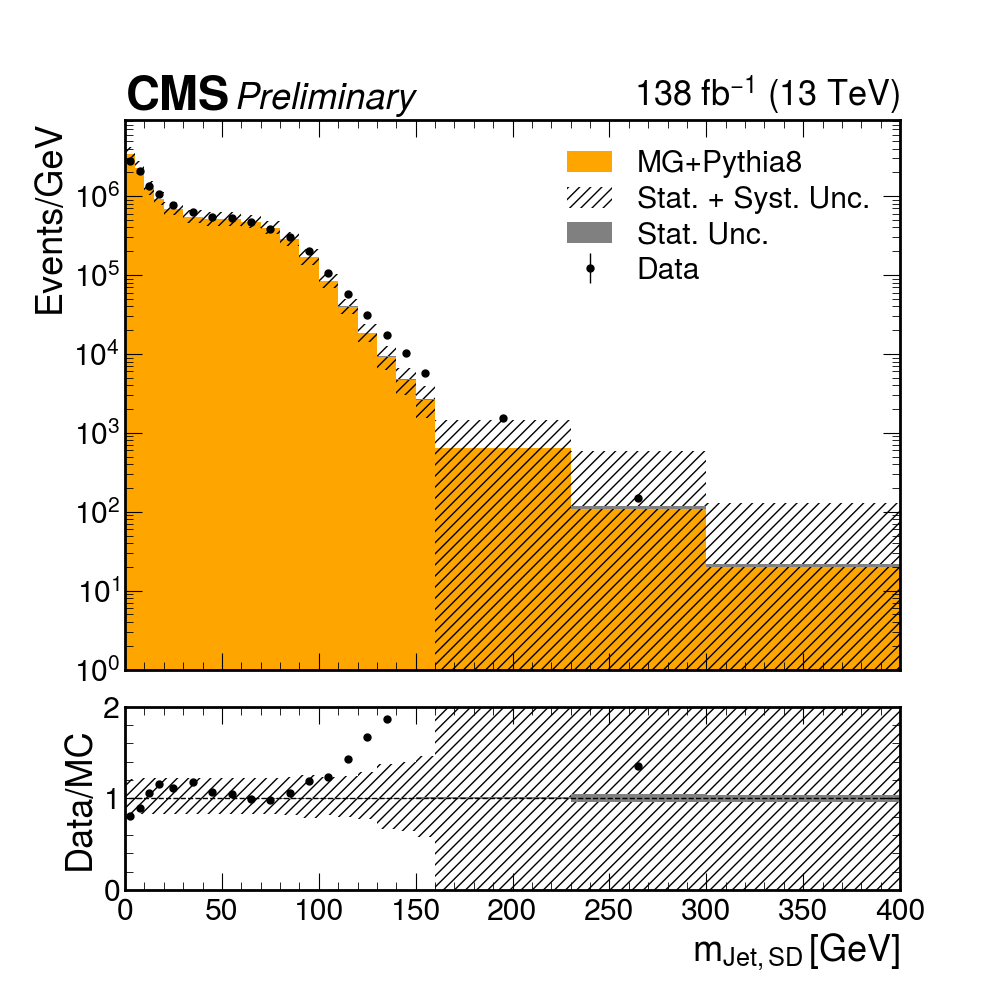
\includegraphics[width=0.45\textwidth]{figures/multijet/trijet/msd_allyears_coarsebin.png}
  \end{subfigure}
  \begin{subfigure}
    \centering
    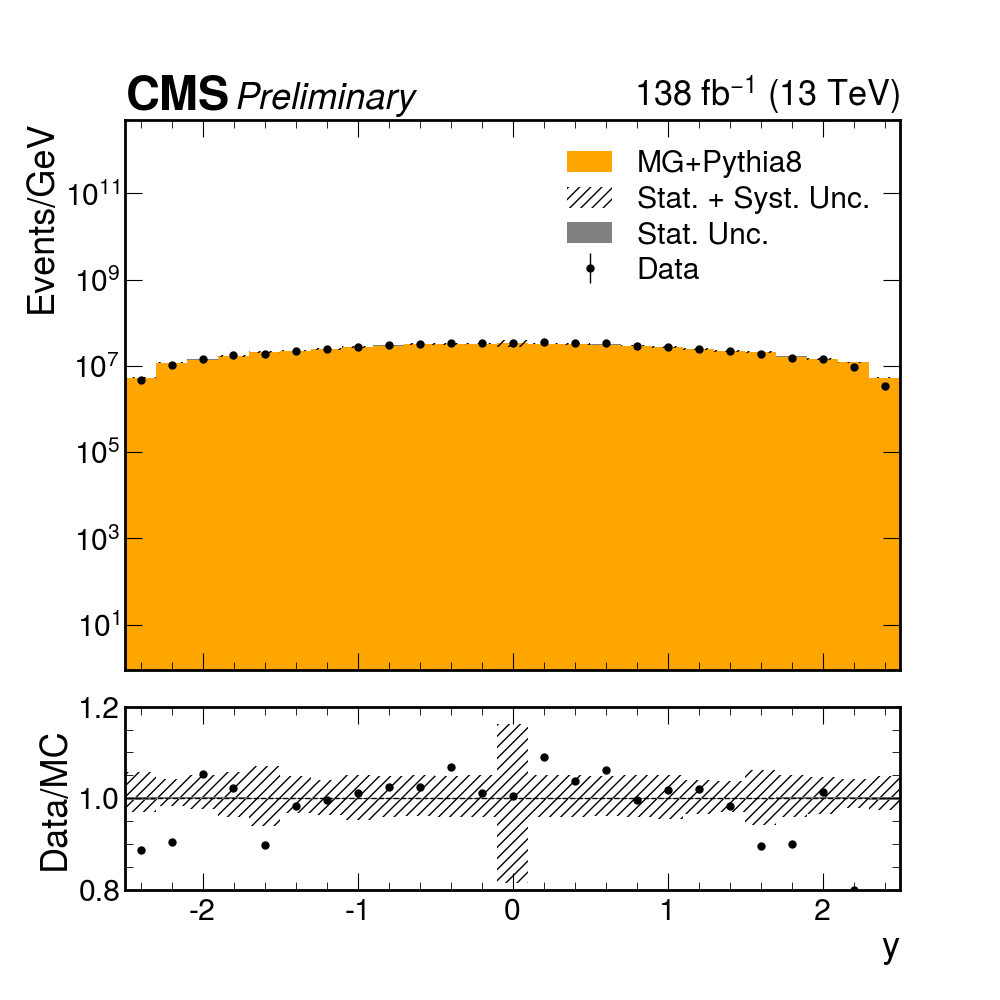
\includegraphics[width=0.45\textwidth]{figures/multijet/trijet/rap_allyears_coarsebin.png}
  \end{subfigure}
  \begin{subfigure}
    \centering
    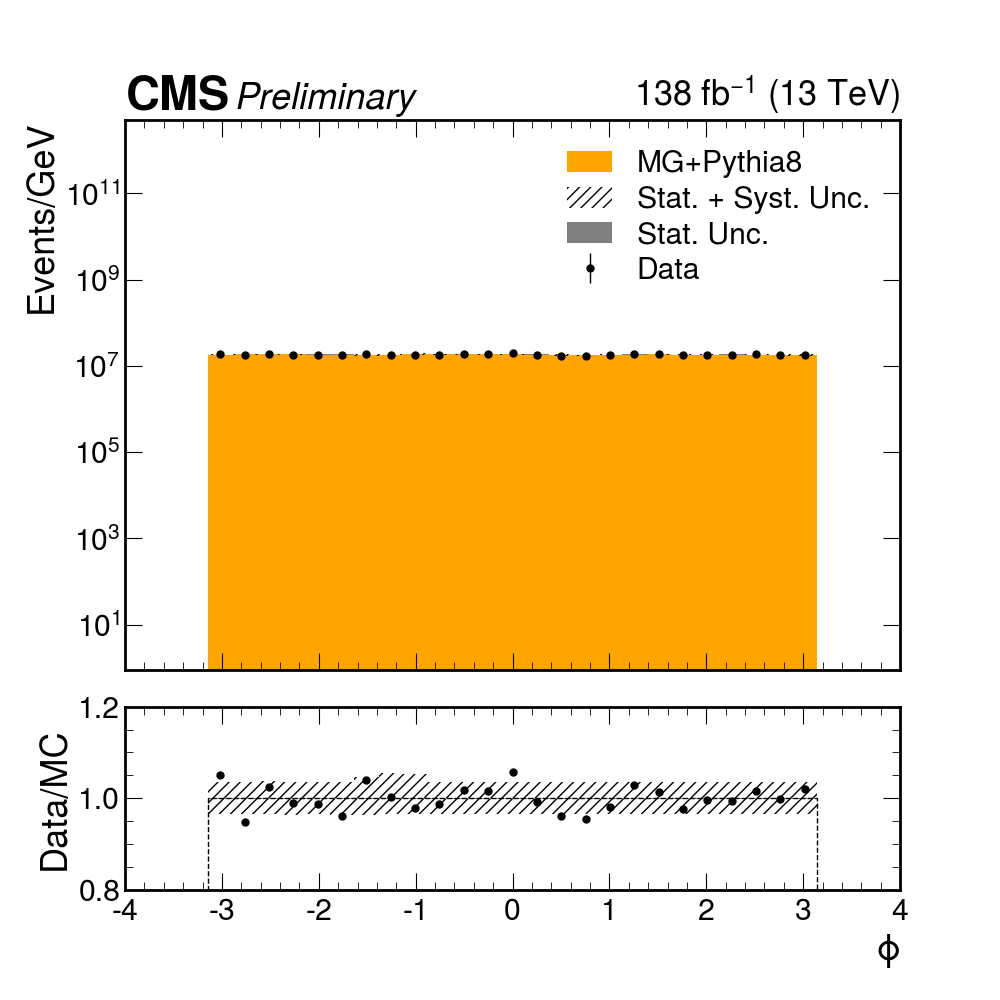
\includegraphics[width=0.45\textwidth]{figures/multijet/trijet/phi_allyears_coarsebin.png}
  \end{subfigure}
  \caption{Full Run 2 UL trijet Data to MC comparison for ungroomed mass (top left), transverse momentum (top right), softdrop mass (center left), rapidity (center right), and phi (bottom).}
  \label{fig:16}
\end{figure}
\begin{figure}[h!]
  \centering
  \begin{subfigure}
    \centering
    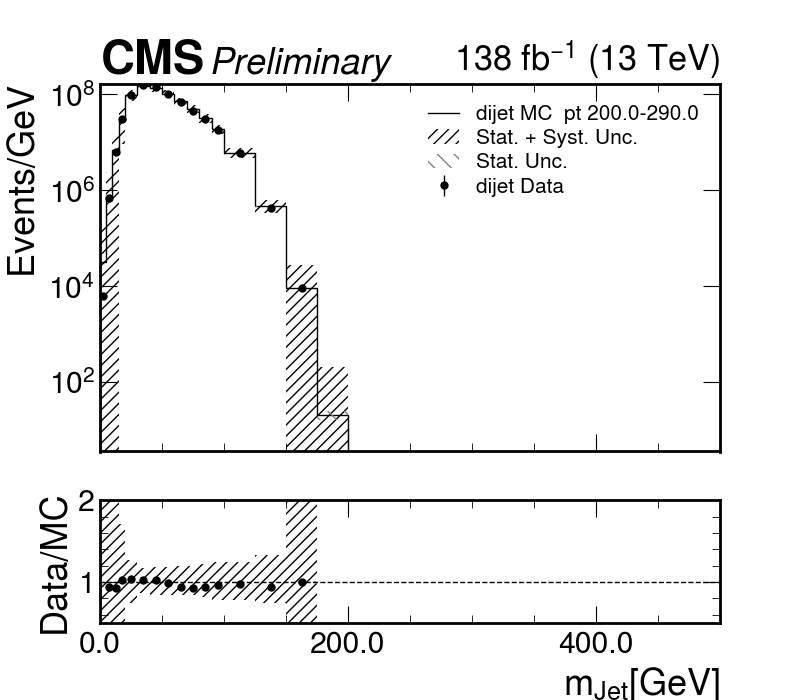
\includegraphics[width=0.45\textwidth]{figures/multijet/dijet/dijet_m_200_290.png}
  \end{subfigure}
  \begin{subfigure}
    \centering
    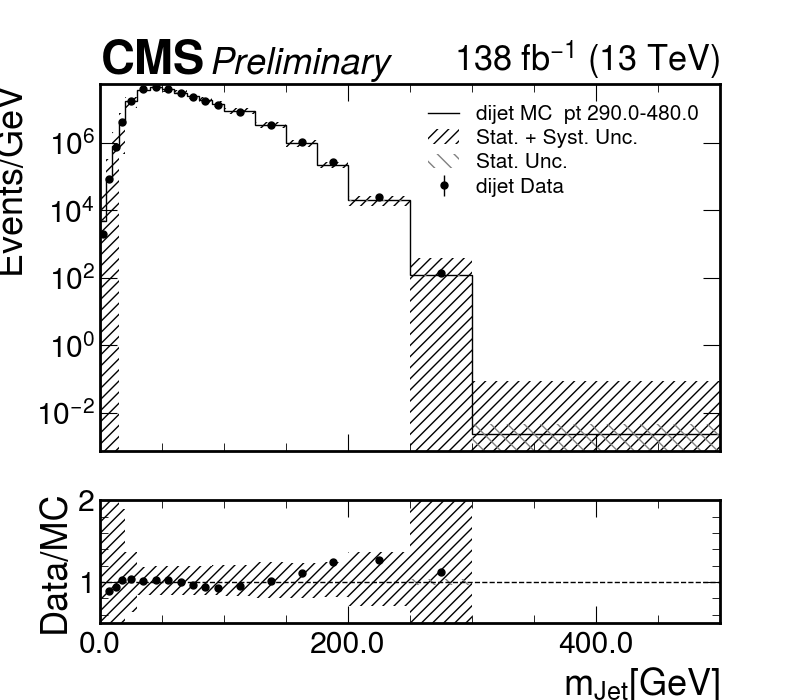
\includegraphics[width=0.45\textwidth]{figures/multijet/dijet/dijet_m_290_480.png}
  \end{subfigure}
  \begin{subfigure}
    \centering
    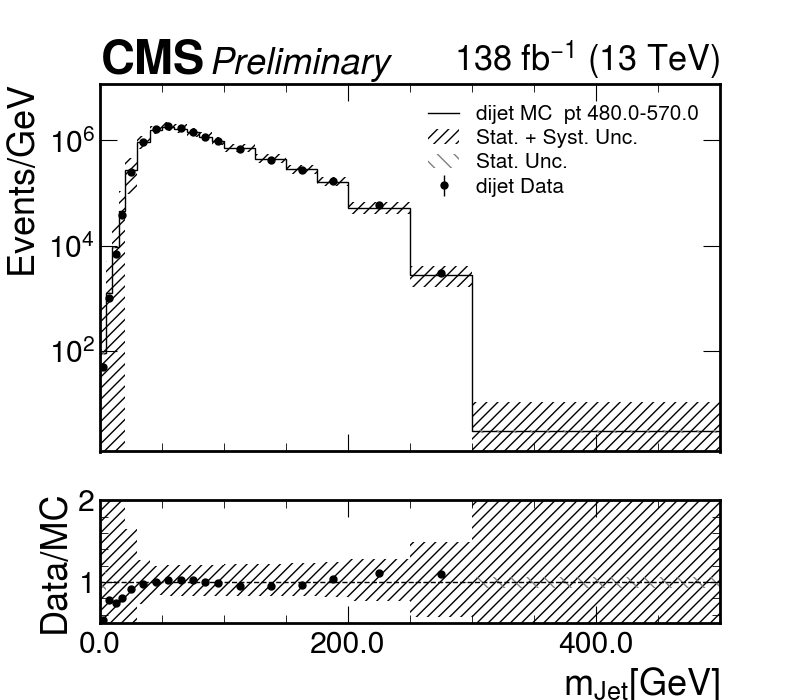
\includegraphics[width=0.45\textwidth]{figures/multijet/dijet/dijet_m_480_570.png}
  \end{subfigure}
  \begin{subfigure}
    \centering
    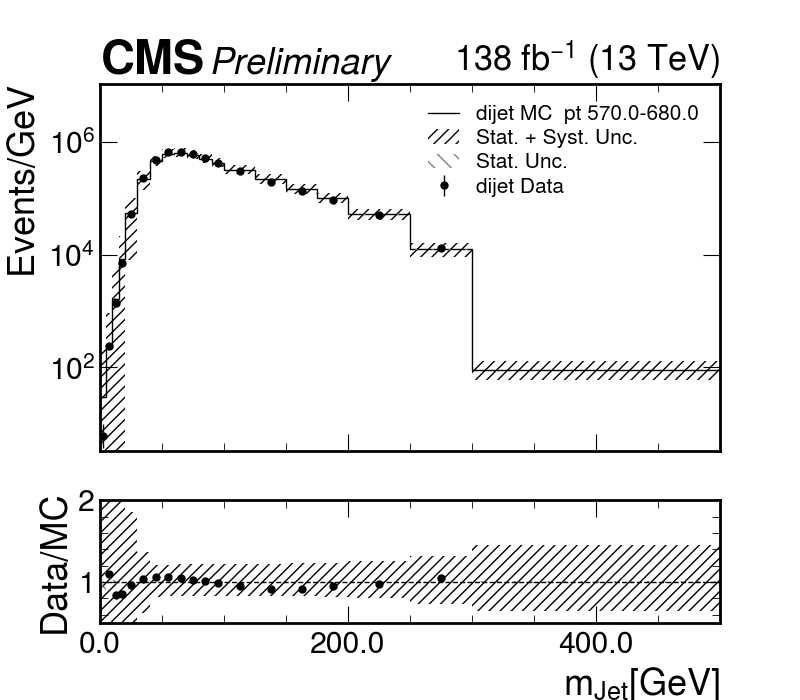
\includegraphics[width=0.45\textwidth]{figures/multijet/dijet/dijet_m_570_680.png}
  \end{subfigure}
  \begin{subfigure}
    \centering
    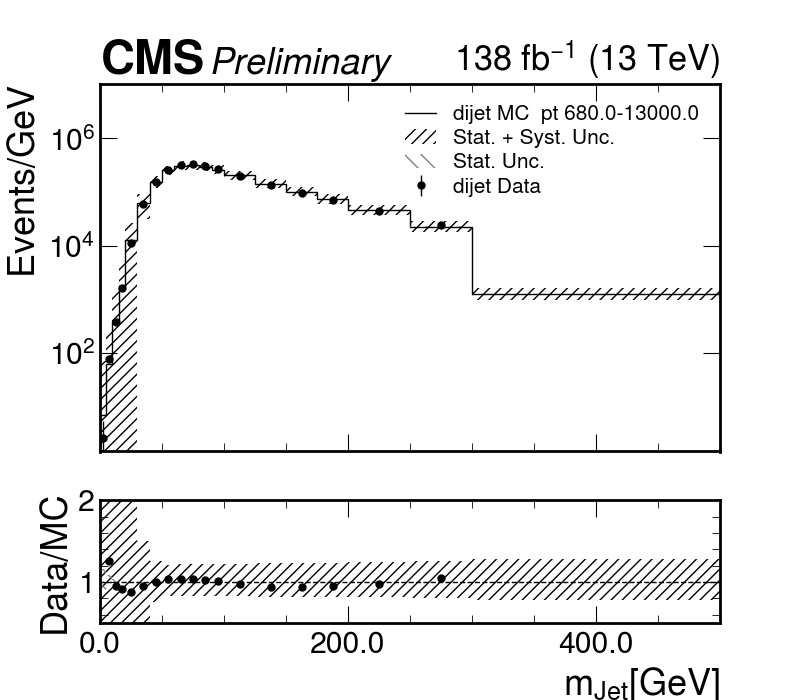
\includegraphics[width=0.45\textwidth]{figures/multijet/dijet/dijet_m_680_13000.png}
  \end{subfigure}
  \caption{Dijet channel  Data to MC comparison for ungroomed mass within each pT bin. MC is normalised to the integral of the data within each \pt bin.}
  \label{fig:17}
\end{figure}
\begin{figure}[h!]
  \centering
  \begin{subfigure}
    \centering
    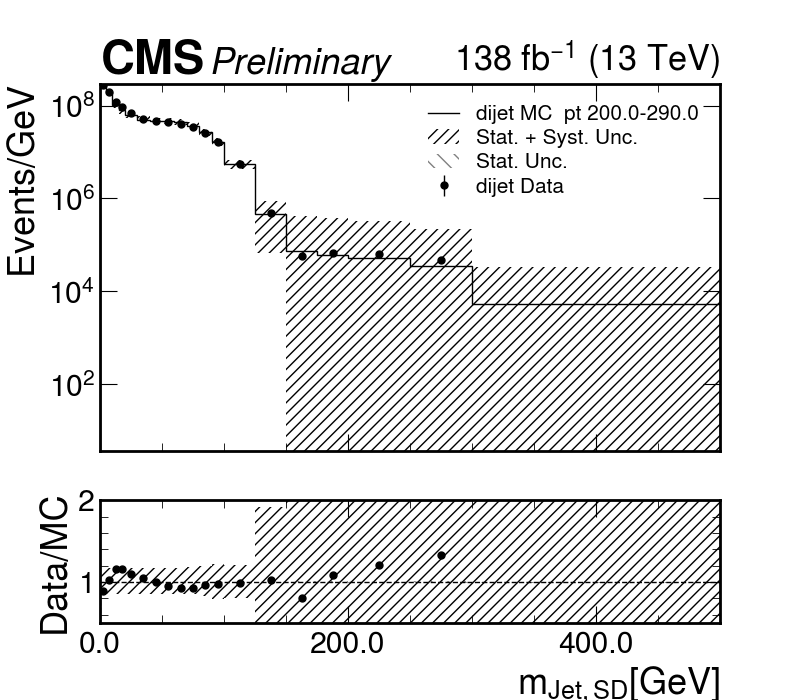
\includegraphics[width=0.45\textwidth]{figures/multijet/dijet/dijet_msd_200_290.png}
  \end{subfigure}
  \begin{subfigure}
    \centering
    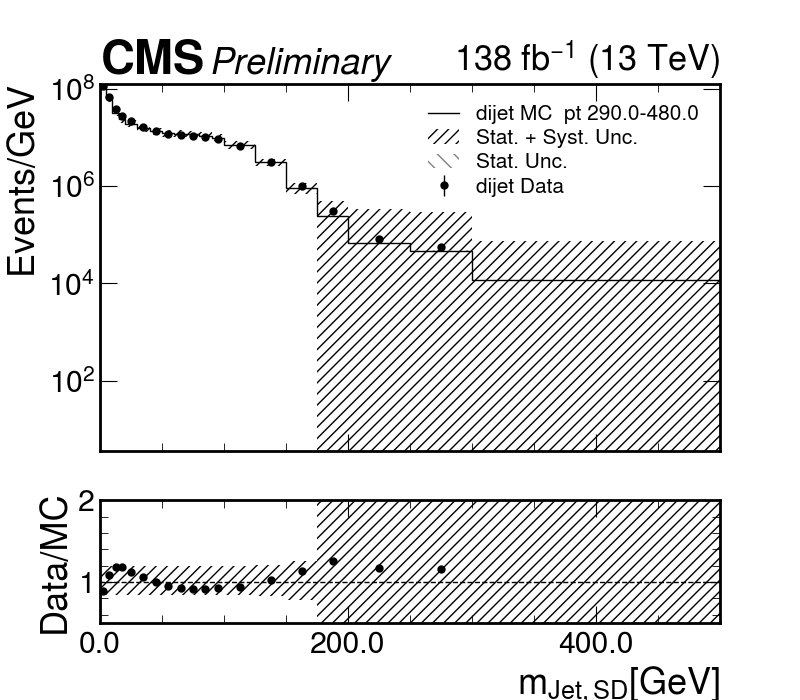
\includegraphics[width=0.45\textwidth]{figures/multijet/dijet/dijet_msd_290_480.png}
  \end{subfigure}
  \begin{subfigure}
    \centering
    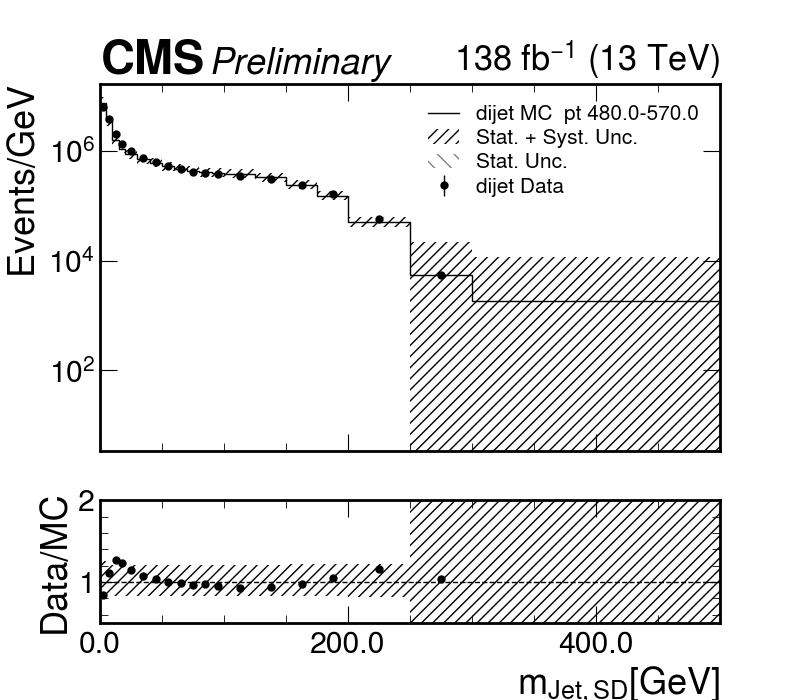
\includegraphics[width=0.45\textwidth]{figures/multijet/dijet/dijet_msd_480_570.png}
  \end{subfigure}
  \begin{subfigure}
    \centering
    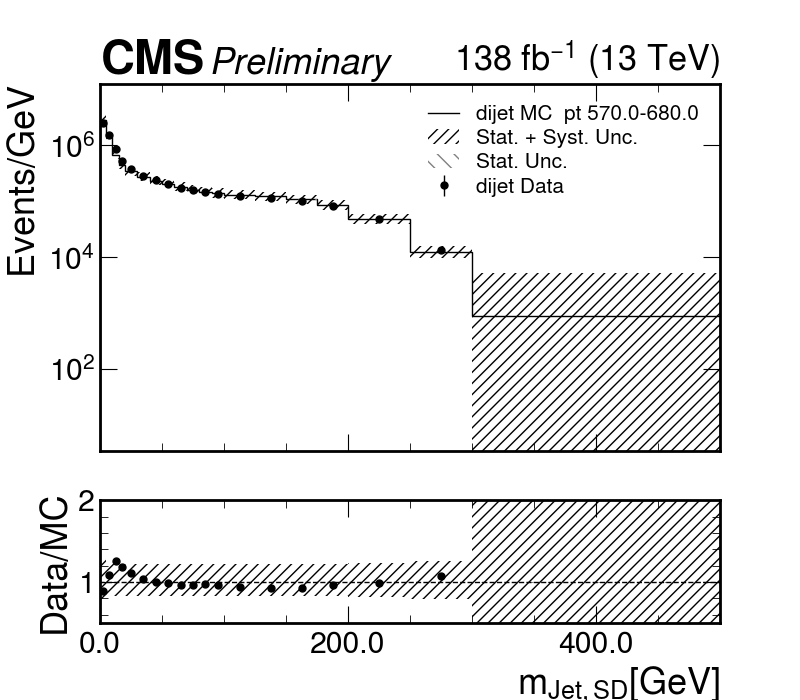
\includegraphics[width=0.45\textwidth]{figures/multijet/dijet/dijet_msd_570_680.png}
  \end{subfigure}
  \begin{subfigure}
    \centering
    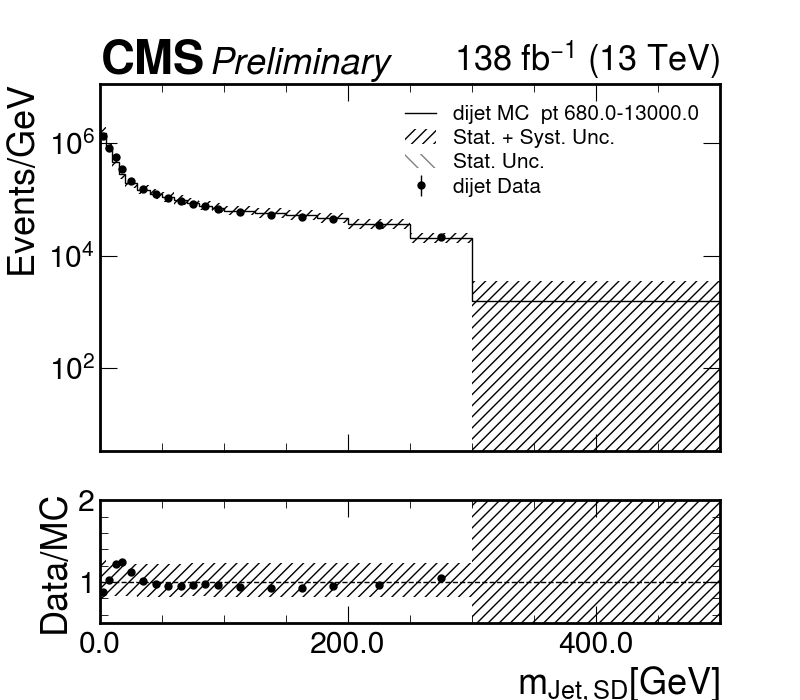
\includegraphics[width=0.45\textwidth]{figures/multijet/dijet/dijet_msd_680_13000.png}
  \end{subfigure}
  \caption{Dijet channel  Data to MC comparison for the softdrop mass within each pT bin. MC is normalised to the integral of the data within each \pt bin.}
  \label{fig:18}
\end{figure}

\begin{figure}[h!]
  \centering
  \begin{subfigure}
    \centering
    
    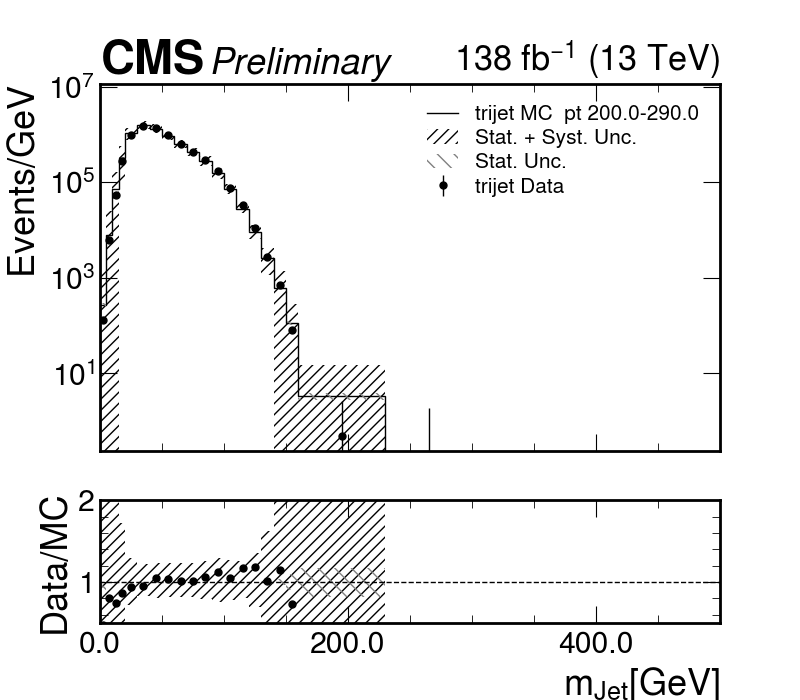
\includegraphics[width=0.45\textwidth]{figures/multijet/trijet/trijet_m_200_290.png}
  \end{subfigure}
  \begin{subfigure}
    \centering
    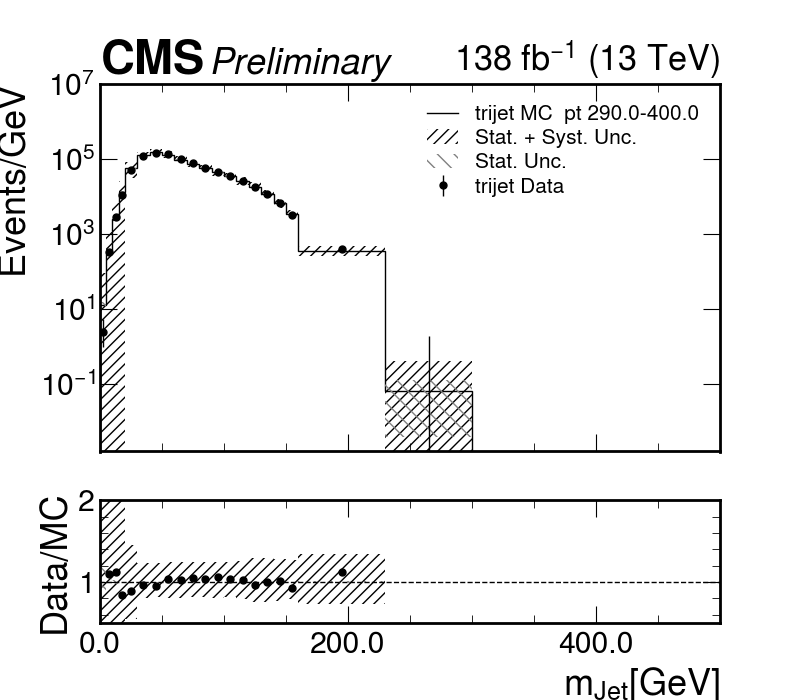
\includegraphics[width=0.45\textwidth]{figures/multijet/trijet/trijet_m_290_400.png}
  \end{subfigure}
  \begin{subfigure}
    \centering
    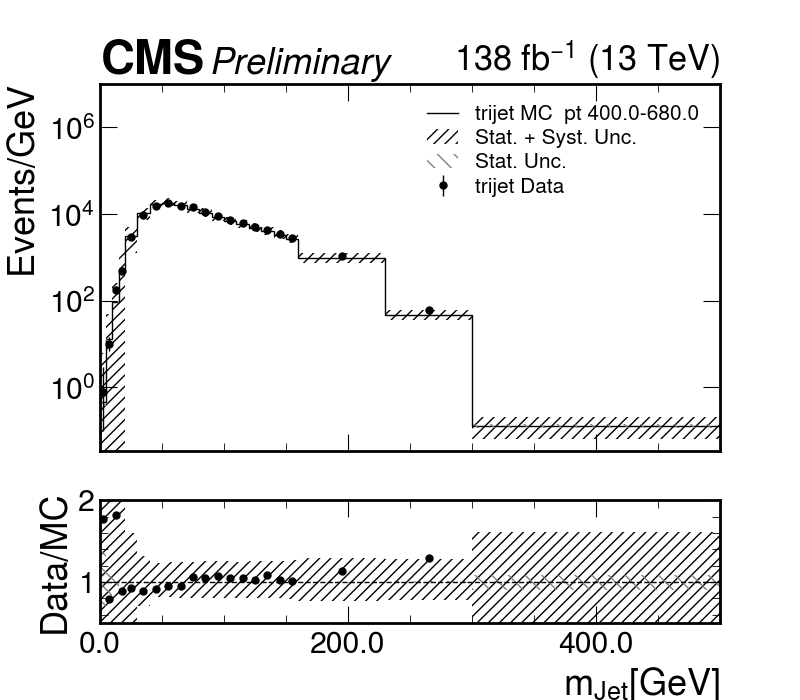
\includegraphics[width=0.45\textwidth]{figures/multijet/trijet/trijet_m_400_680.png}
  \end{subfigure}
  \begin{subfigure}
    \centering
    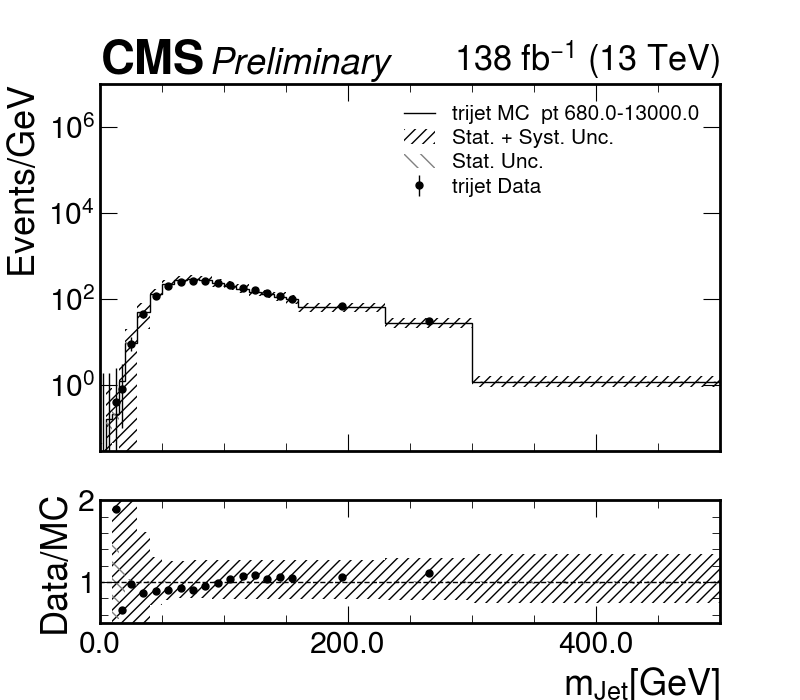
\includegraphics[width=0.45\textwidth]{figures/multijet/trijet/trijet_m_680_13000.png}
  \end{subfigure}
  \caption{Trijet channel  Data to MC comparison for ungroomed mass within each pT bin. MC is normalised to the integral of the data within each \pt bin.}
  \label{fig:19}
\end{figure}
\begin{figure}[h!]
  \centering
  \begin{subfigure}
    \centering
    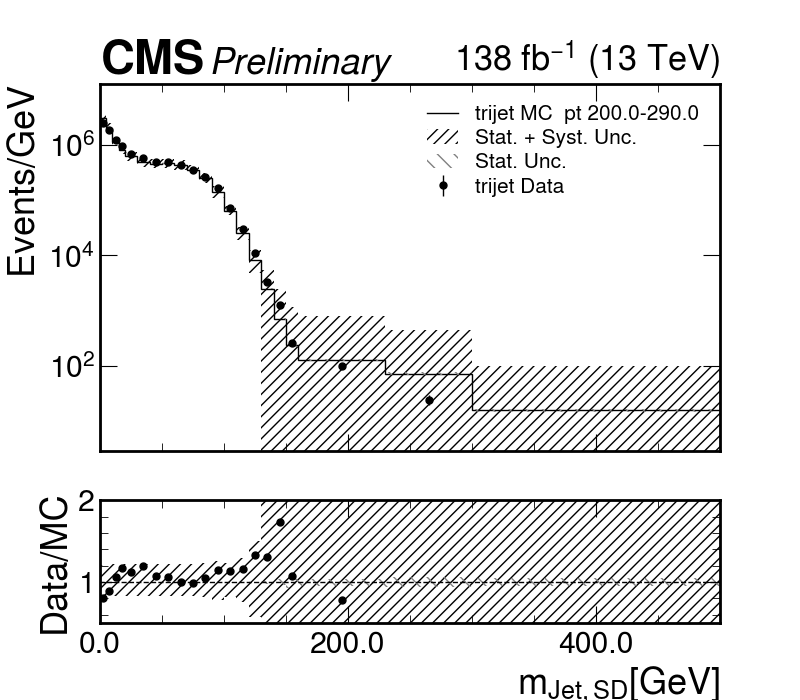
\includegraphics[width=0.45\textwidth]{figures/multijet/trijet/trijet_msd_200_290.png}
  \end{subfigure}
  \begin{subfigure}
    \centering
    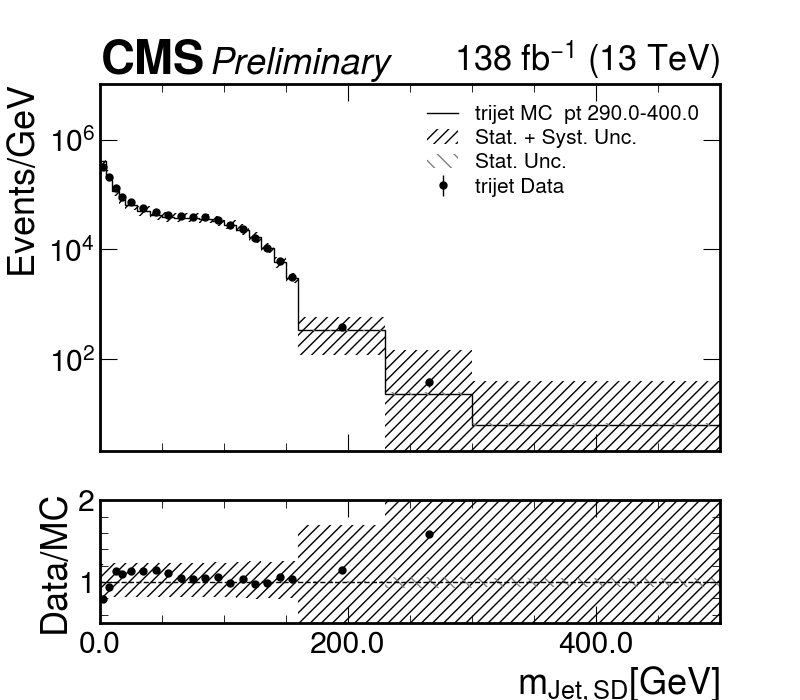
\includegraphics[width=0.45\textwidth]{figures/multijet/trijet/trijet_msd_290_400.png}
  \end{subfigure}
  \begin{subfigure}
    \centering
    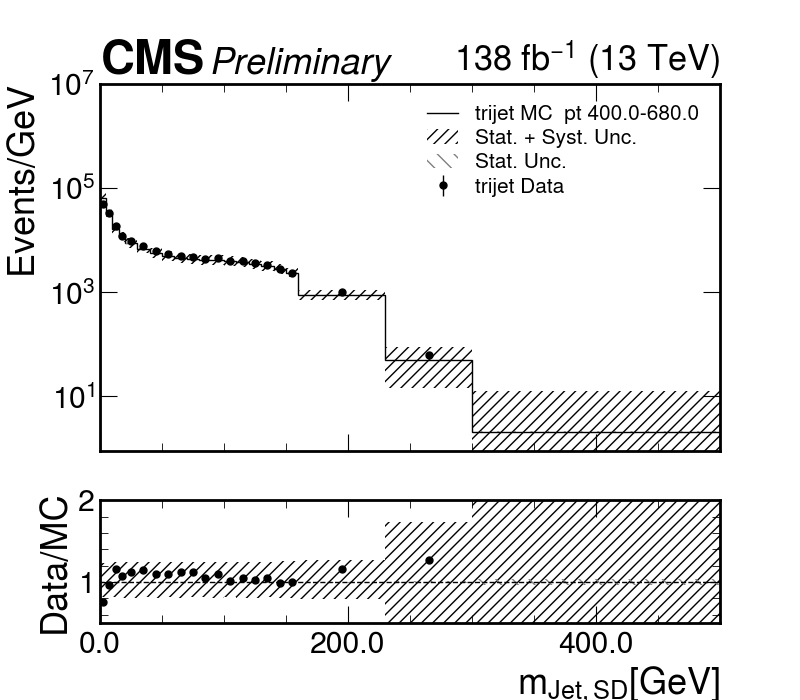
\includegraphics[width=0.45\textwidth]{figures/multijet/trijet/trijet_msd_400_680.png}
  \end{subfigure}
  \begin{subfigure}
    \centering
    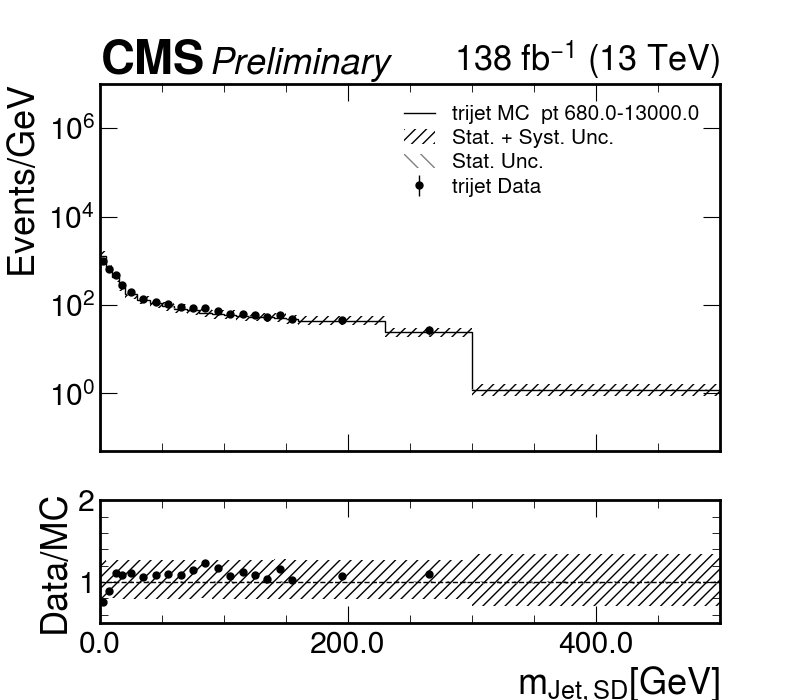
\includegraphics[width=0.45\textwidth]{figures/multijet/trijet/trijet_msd_680_13000.png}
  \end{subfigure}
  \caption{Trijet channel  Data to MC comparison for the softdrop mass within each pT bin. MC is normalised to the integral of the data within each \pt bin.}
  \label{fig:20}
\end{figure}


\section{Uncertainties}
The reconstructed events in this analysis are subject to statistical and systematic uncertainties that must be propagated through the unfolding to the final measurement.
\subsection{Statistical Uncertainty}
To estimate the statistical uncertainty after unfolding, the jackknife resampling method is employed \cite{economics_jk}. This method is helpful in estimating the variance of a limited sample set and is computed by finding the mean of $N$ independent subsamples of size $N-1$ of the dataset and weighting that by $\sqrt{N/N-1}$. In our case, this means producing N separate response matrices using a fraction $(N-1)/N$ of the data for each response matrix, leaving an independent $1/N-1$ fraction of events out of each matrix. The unfolded cross-section is computed for each of these response matrices and the final statisitical uncertainty for the total result is taken as
\begin{equation}
  \label{eq:jk}
  \sigma_{stat} = \sqrt{\frac{N}{N-1}}\sigma
\end{equation}
where $\sigma$ is the standard deviation of the N unfolded variations and $\sigma_{stat}$ is taken as the statistical uncertainty. In this analysis we used $N=10$ subsamples to compute the statistical uncertainty and the spread of these unfolded subsamples can be seen in figure \ref{fig:jk}.

\subsection{Systematic Uncertainties}
The sources of systematic uncertainties affecting this analysis are described in this section. Since the data is split into 4 distinct eras, the correlations of the uncertainties between the eras is also described.
\begin{itemize}
\item \textbf{Jet Energy Scale (JES)} Uncertainties associated with the JECs, as described in section \ref{JEC}, are derived by varying the scale by $\pm 1 \sigma$ for each individual uncertainty source. There are 27 uncertainty sources per year and their correlations between years are provided by the CMS collaboration \cite{JEC}. The correlation between years for each uncertainty source is shown in Table \ref{table:tab2}. For simplicity, given a correlation factor $\rho$ and a variation $\sigma$ , the correlated part $\sigma_{corr}$ and uncorrelated part of the variation $\sigma_{uncorr}$ are given by:
  \begin{equation}
    \label{eq:corr}
    \sigma_{corr}=\sigma\rho
  \end{equation}
    \begin{equation}
    \label{eq:uncorr}
    \sigma_{uncorr}=(1-\rho)\sigma
  \end{equation}
  Each uncertainty variation is considered in a separate response matrix and unfolded separately.
  \begin{table}[h!]
    \centering
    \begin{tabular}{lr}
      \hline
      Uncertainty & Correlation \\ \hline
      AbsoluteMPFBias & 100\% \\
      AbsoluteScale & 100\% \\
      AbsoluteStat & 0\% \\
      FlavorQCD & 100\% \\
      Fragmentation & 100\% \\
      PileUpDataMC & 50\% \\
      PileUpPtBB & 50\% \\
      PileUpPtEC1 &50\% \\
      PileUpPtEC2 & 50\% \\
      PileUpPtHF & 50\% \\
      PileUpPtRef & 50\% \\
      RelativeFSR & 50\% \\
      RelativeJEREC1 & 0\% \\
      RelativeJEREC2 & 0\% \\
      RelativeJERHF & 50\% \\
      RelativePtBB & 50\% \\
      RelativePtEC1 & 0\% \\
      RelativePtEC2 & 0\% \\
      RelativePtHF & 50\% \\
      RelativeBal & 50\% \\
      RelativeSample & 0\% \\
      RelativeStatEC & 0\% \\
      RelativeStatFSR & 0\% \\
      RelativeStatHF & 0\% \\
      SinglePionECAL & 100\% \\
      SinglePionHCAL & 100\% \\
      TimePtEta & 0\% \\ \hline
    \end{tabular}
    \caption{Correlations between data taking periods for all JEC uncertainty sources.}
    \label{table:tab2}
  \end{table}
\item \textbf{Jet Energy Resolution (JER):} Similar to the JES uncertainties, the JER uncertainty is a $1\sigma$ shift and fully correlated in  \pt and $\eta$ and uncorrelated across years. Again, these uncertainty values are provided by the CMS Collaboartion \cite{JEC}.
\item \textbf{Jet Mass Scale (JMS) and Resolution (JMR)} Just like the JES and JER uncertainties, the JMS and JMR uncertainties are calculated as a 1 sigma shift (?). These values are again provided by the collaboration and can be seen in the \ref{table:JMS}.
\item \textbf{Integrated Luminosity:}
 The uncertainty on the measurement of the full Run II luminosity$\script{L}_{int}\approx 137.2 fb^{-1}$ is estimated to be 1.6\% \cite{lumi2016, lumi2017, lumi2018}. This uncertainty is accounted for as its own response matrix and normalized post unfolding.
\item \textbf{Pileup Re-weighting:}
 As decribed in \ref{PUSF}, simulation samples are reweighted to match the pileup profile in data from the using the number of interactions per bunch crossing. This is estimated from measurements of the luminosity and the inclusive cross section for Run II $\sigma^{inel}_{pp} = 69.2 mb$ \cite{LUMIPOGtwiki}. The corresponding uncertainty is calculated by varying the total inelastic cross section by $\pm 4.6\%$ and repeating the reweighting. The uncertainties are treated as fully correlated between data taking eras.
\item \textbf{Parton Distribution Functions (PDFs):}
  The simulated samples contain per-event weights for 100 variations of the original NNPDF3.1 PDF set \cite{nnpdf3.1}. The corresponding systematic uncertainty is taken as the RMS deviation of the variations.
\item \textbf{$q^2$ Scales:}
  The simulated samples contain weights that correspond to variations in the in the factorisation, $\mu_F$ and renormalisation $\mu_R$ scales. The scales are each varied separately by factors of 0.5 and 2 separately, giving 9 permutations in total. Three of these cases are not considered since they vary the scales in the opposite direction, which is unphysical. The other 6 variations (both varied by 2, both varied by 0.5, $\mu_f$ varied up while $\mu_R$ is nominal and vice versa, and  $\mu_f$ varied down while $\mu_R$ is nominal and vice versa) are used to calculate the total scale uncertainty using the envelope method, where the largest observed deviation from the nominal $q^2$ setting is taken as the systematic uncertainty.
\item \textbf{L1 Prefiring:}
  As described in section \ref{prefiring}, during 2016 and 2017 data-taking, there was an additional inefficiency due to an issue in the L1 prefiring. This is corrected for using weights provided by the collaboration. The uncertainties are also provided by the collaboration, and are calculated by shifting the prefiring probabilities by the squared sum of $20\%$ of the prefiring probability and the statistical uncertatinty in each considered bin used to make the pefiring map \cite{l1prefiring}.
\item \textbf{Parton Shower and Hadronization Model}
  We use a separate MG+HERWIG sample to model the effects of the parton shower and hadronisation model. We create a separate response matrix using this model just as we do with each other uncertainty mentioned, unfold the data using it, and include it as an uncertainty. The difference between the herwig and pythia distributions can be seen in figure \ref{fig:herwig}. The resulting uncertainty after unfolding can be seen in the plots in the right column of figures \ref{fig:dijetunc} and \ref{fig:trijetunc}.
  % \item \textbf{HEM} --> not needed if we're veto-ing HEM events
  All of the above uncertainties can be be seen before unfolding and for the ungroomed mass for the dijet(trijet) channel in figure \ref{fig:dijetunc_ungroomed}(\ref{fig:trijetunc_ungroomed}, beforand after unfolding for the ungroomed mass in the dijet(trijet) channel in figure \ref{fig:dijetunc_ungroomed_postunfold}(\ref{fig:trijetunc_ungroomed_postunfold}). For the groomed mass, the uncertainties before unfolding in the dijet(trijet) channel can be seen in figure \ref{fig:dijetunc_groomed}(\ref{fig:trijetunc_groomed}), and after unfolding in figure \ref{fig:dijetunc_groomed_postunfold}(\ref{fig:trijetunc_groomed_postunfold}).
\end{itemize}
\begin{figure}[ht!]
  \centering
  \begin{subfigure}
    \centering
    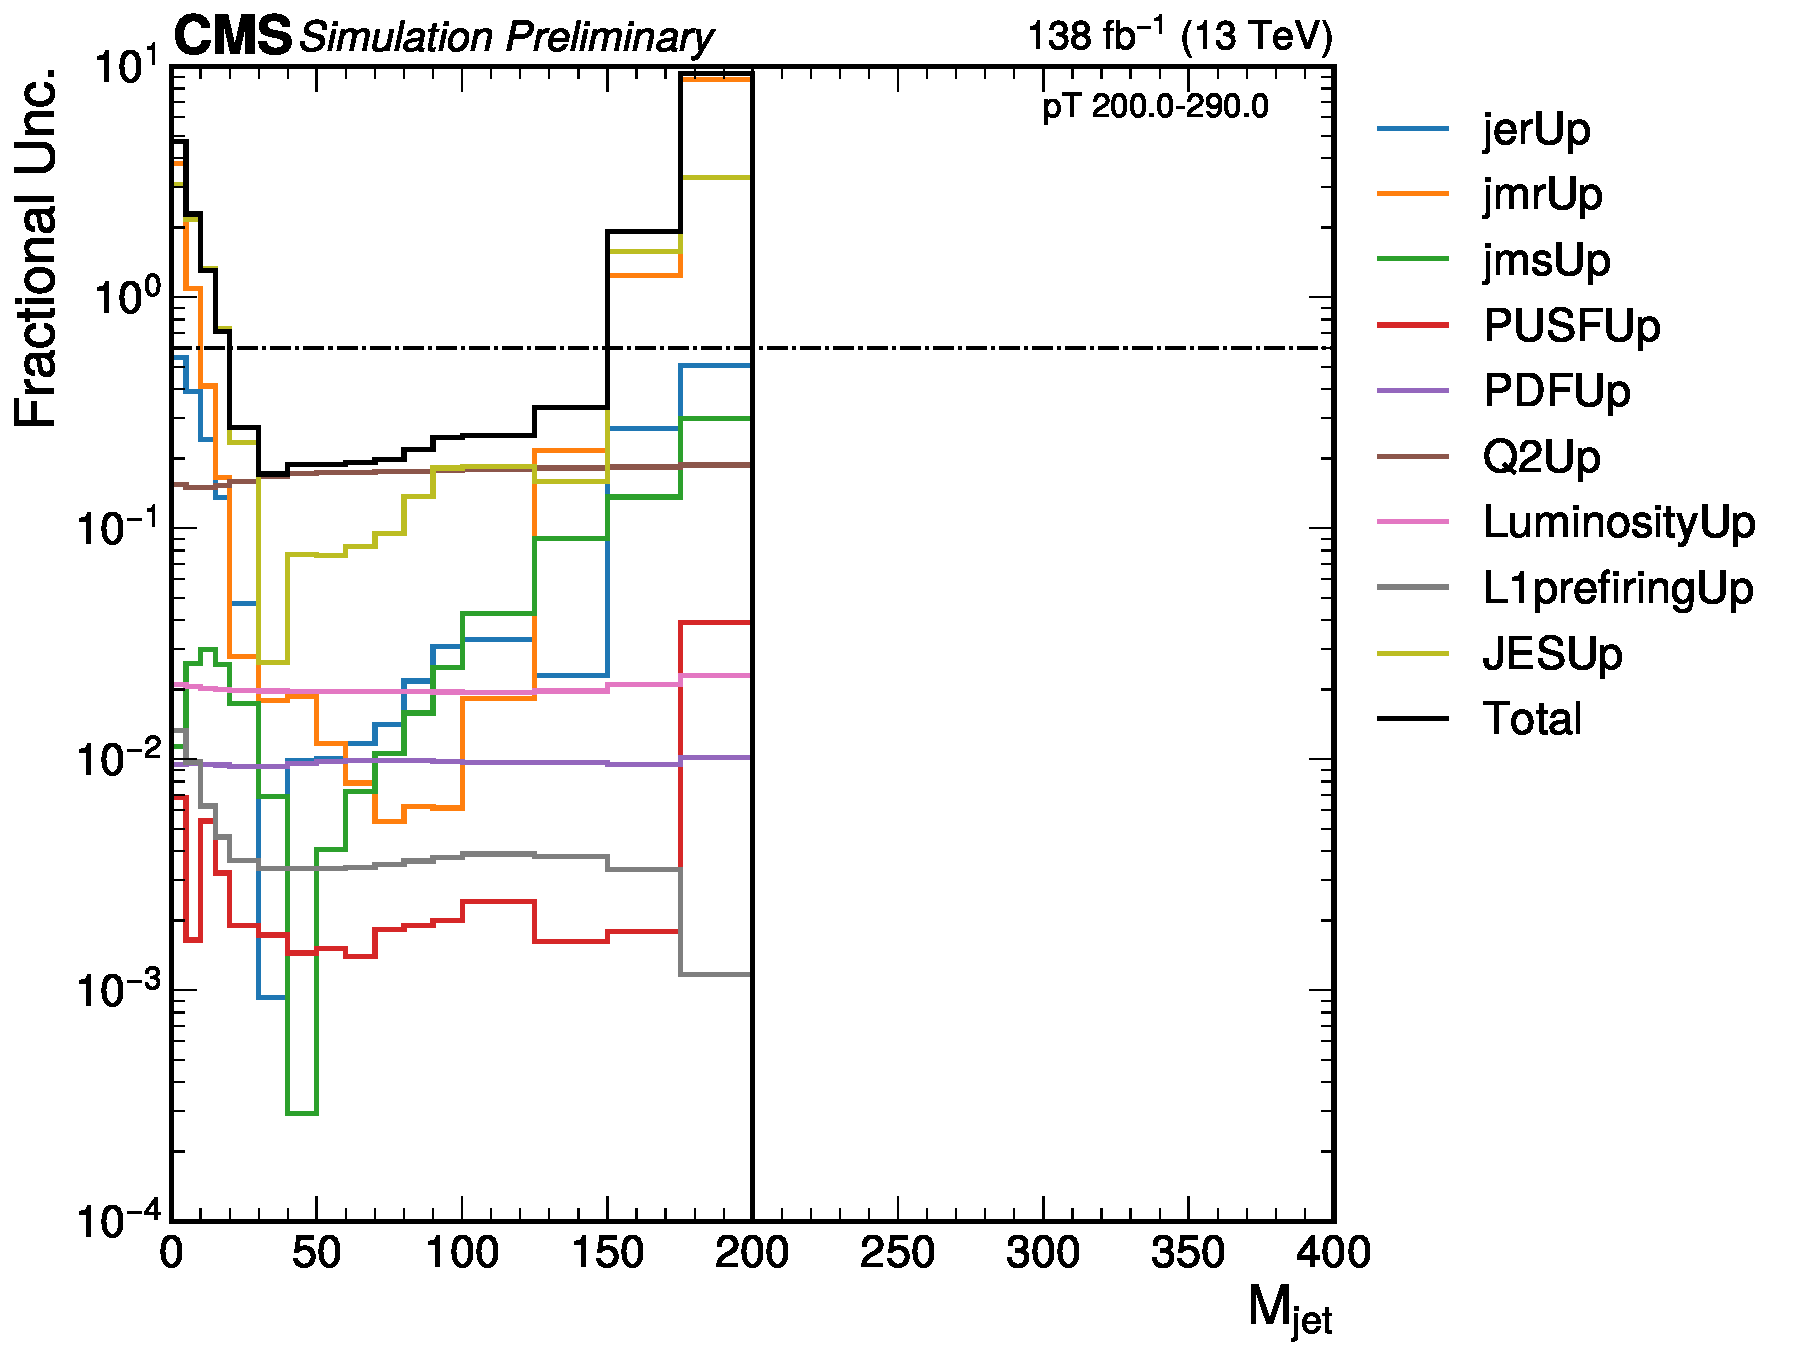
\includegraphics[width=0.45\textwidth]{figures/multijet/dijet/fracUnc_ungroomed_0.pdf}
\end{subfigure} 
  \begin{subfigure}
    \centering
    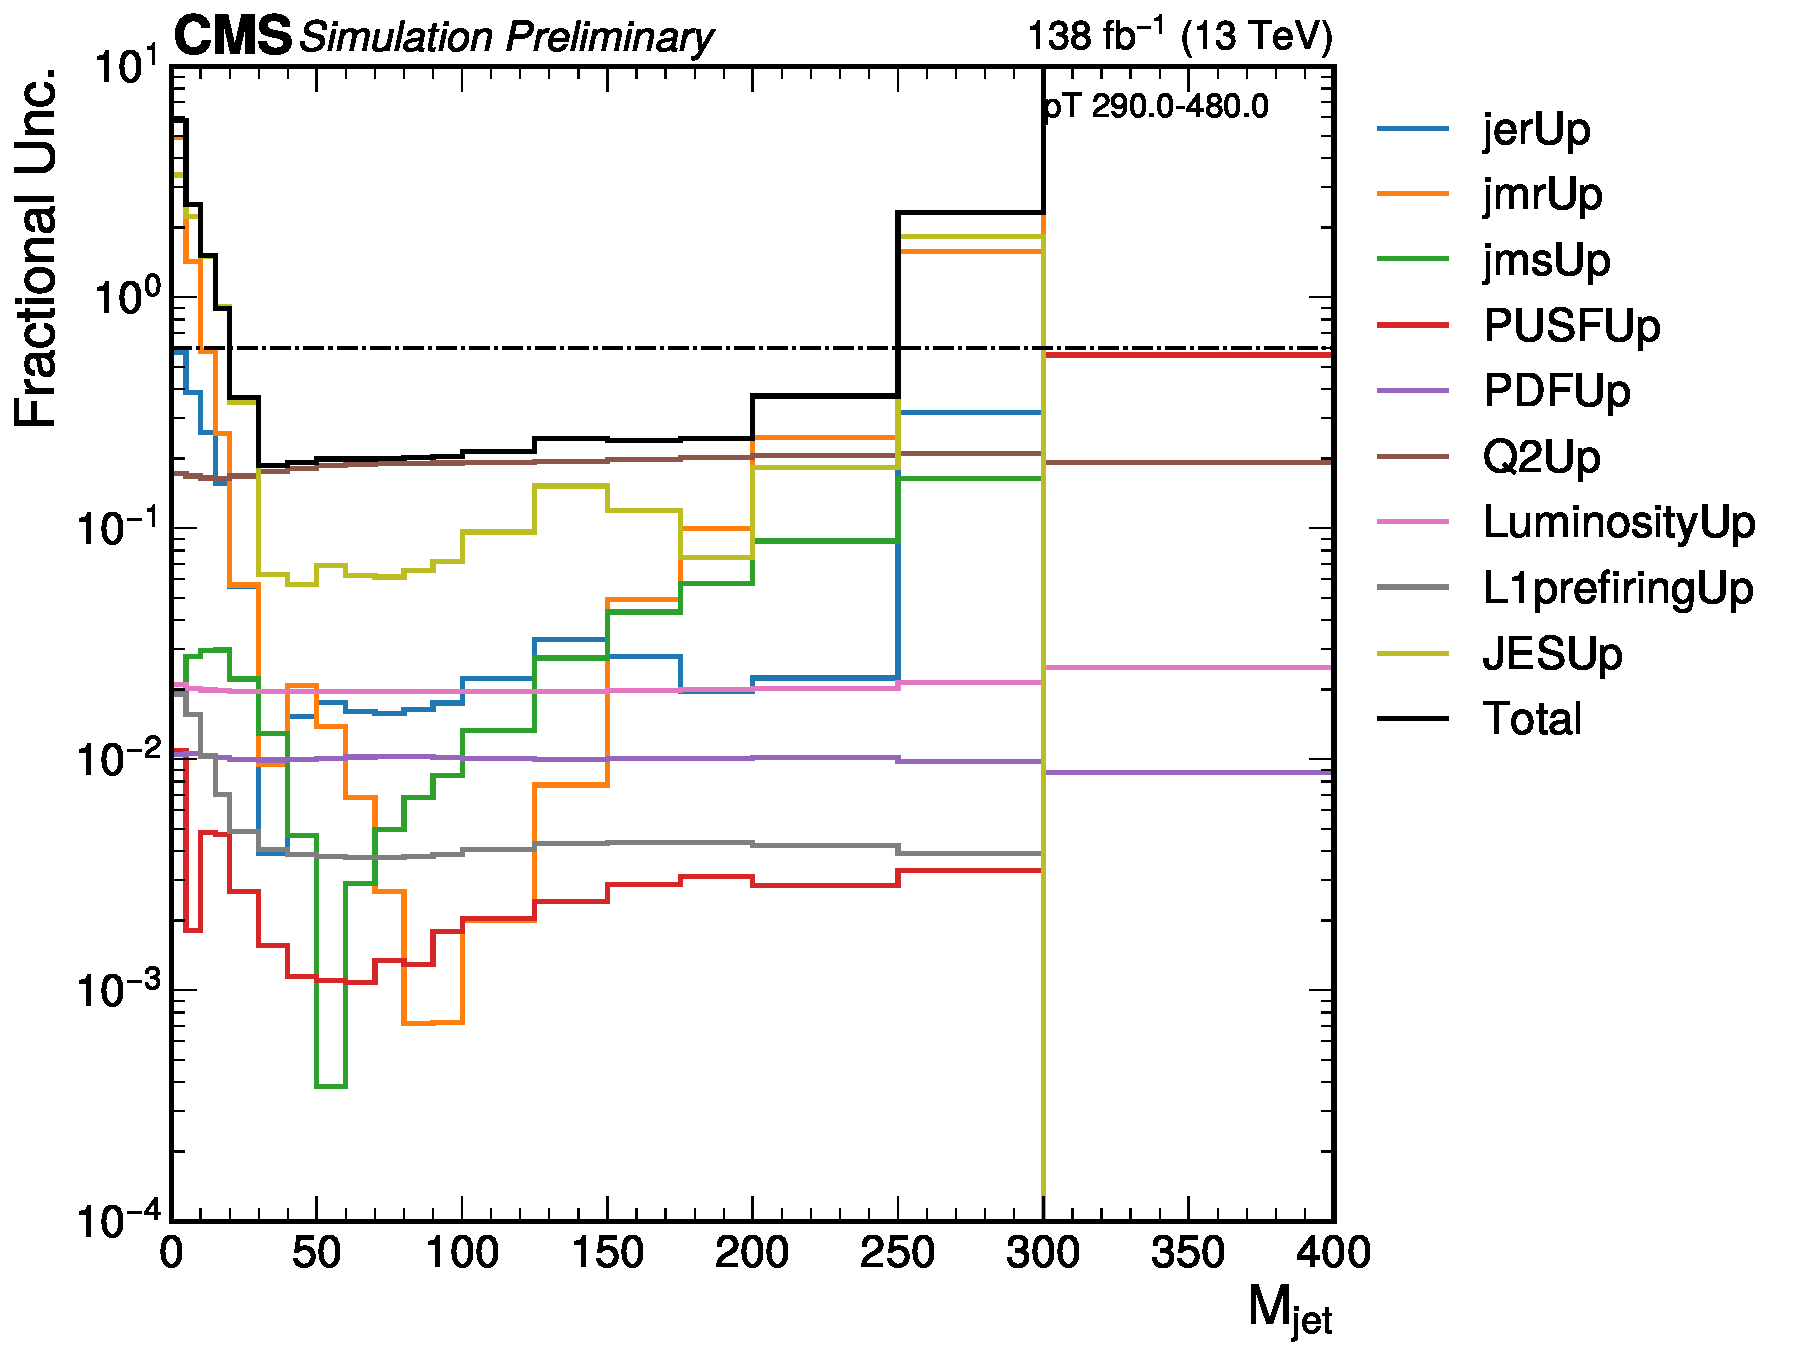
\includegraphics[width=0.45\textwidth]{figures/multijet/dijet/fracUnc_ungroomed_1.pdf}
\end{subfigure}
  \begin{subfigure}
    \centering
    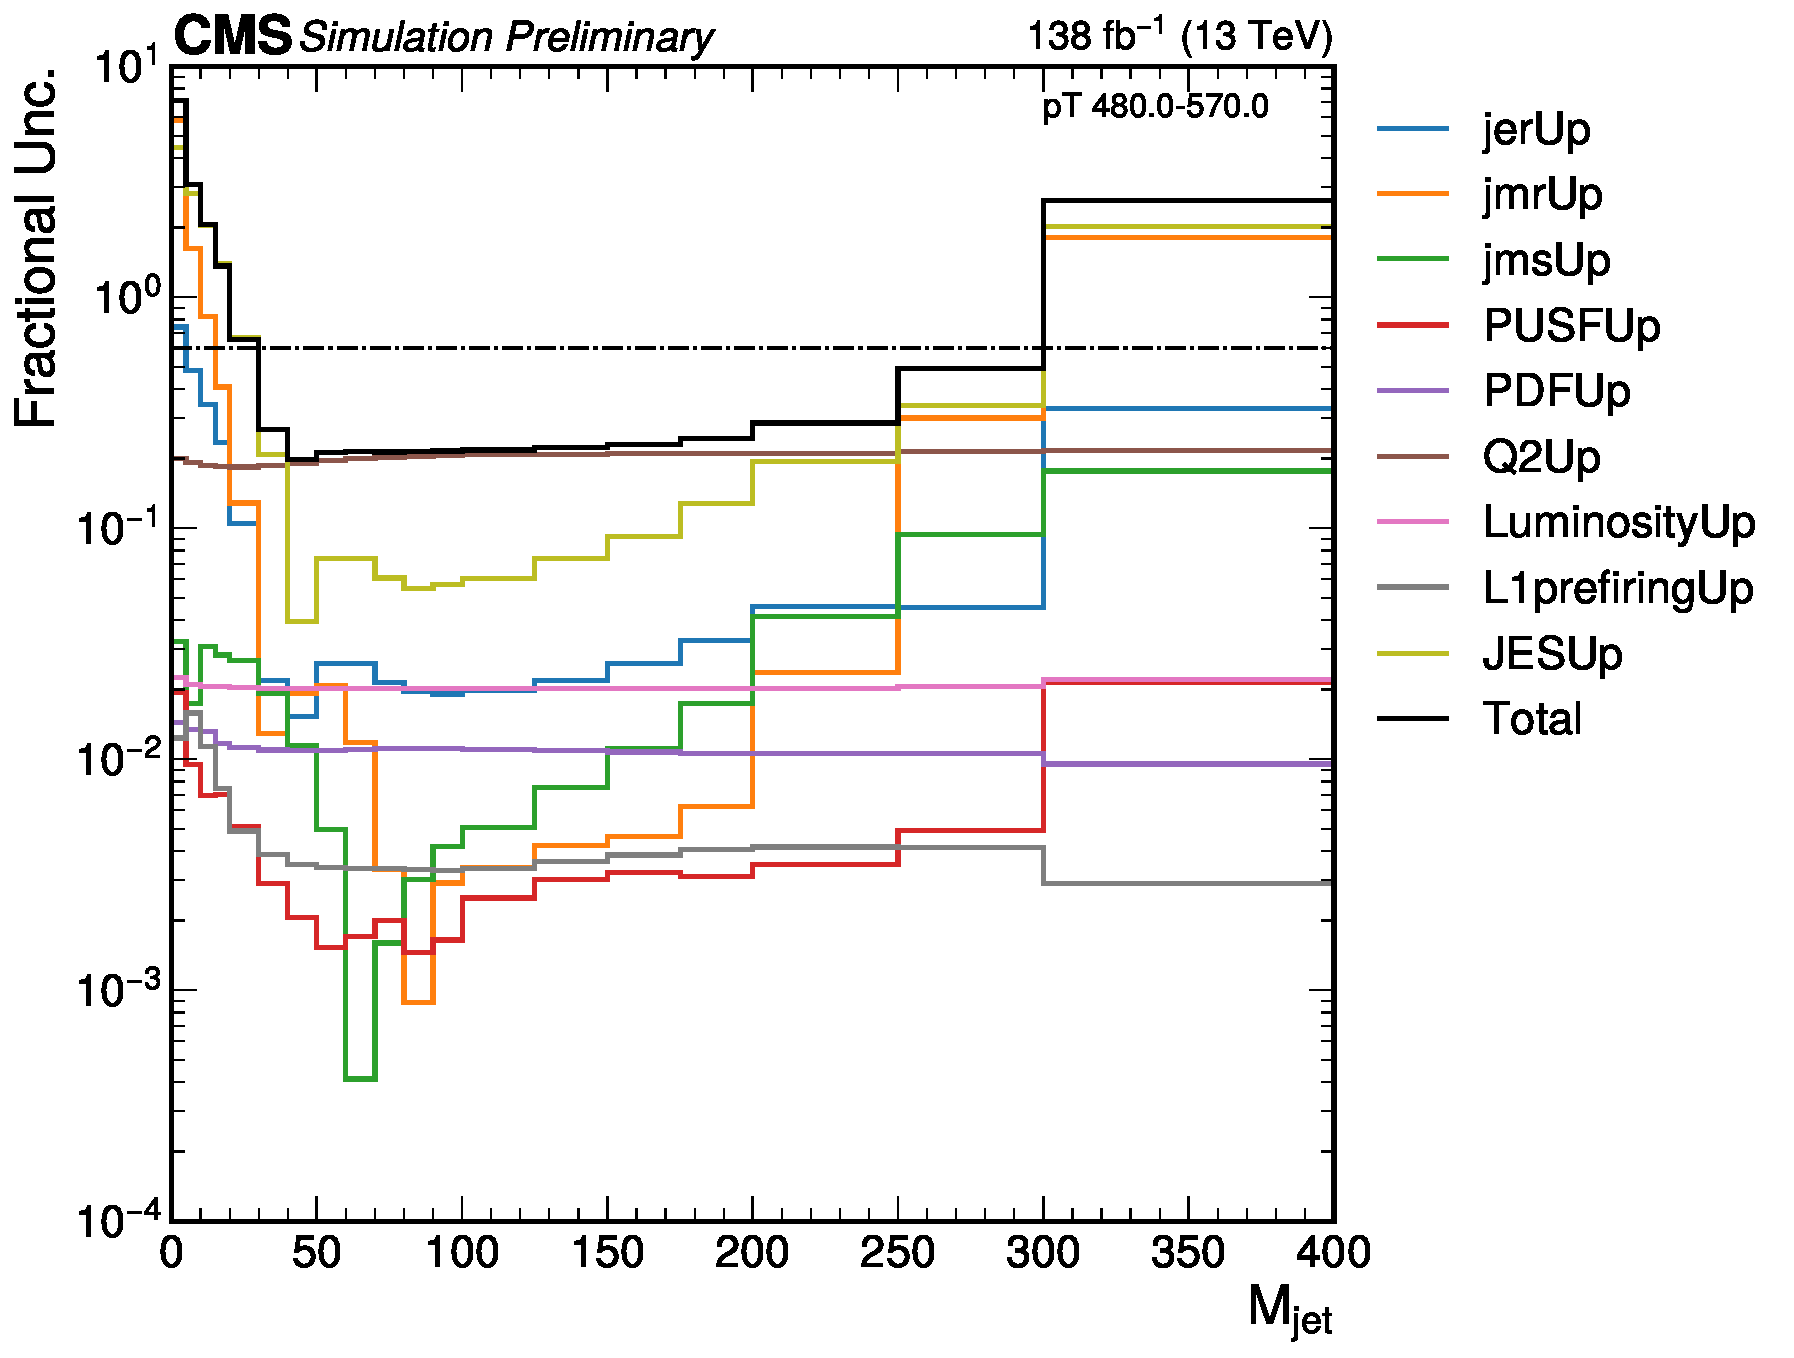
\includegraphics[width=0.45\textwidth]{figures/multijet/dijet/fracUnc_ungroomed_2.pdf}
\end{subfigure}
  \begin{subfigure}
    \centering
    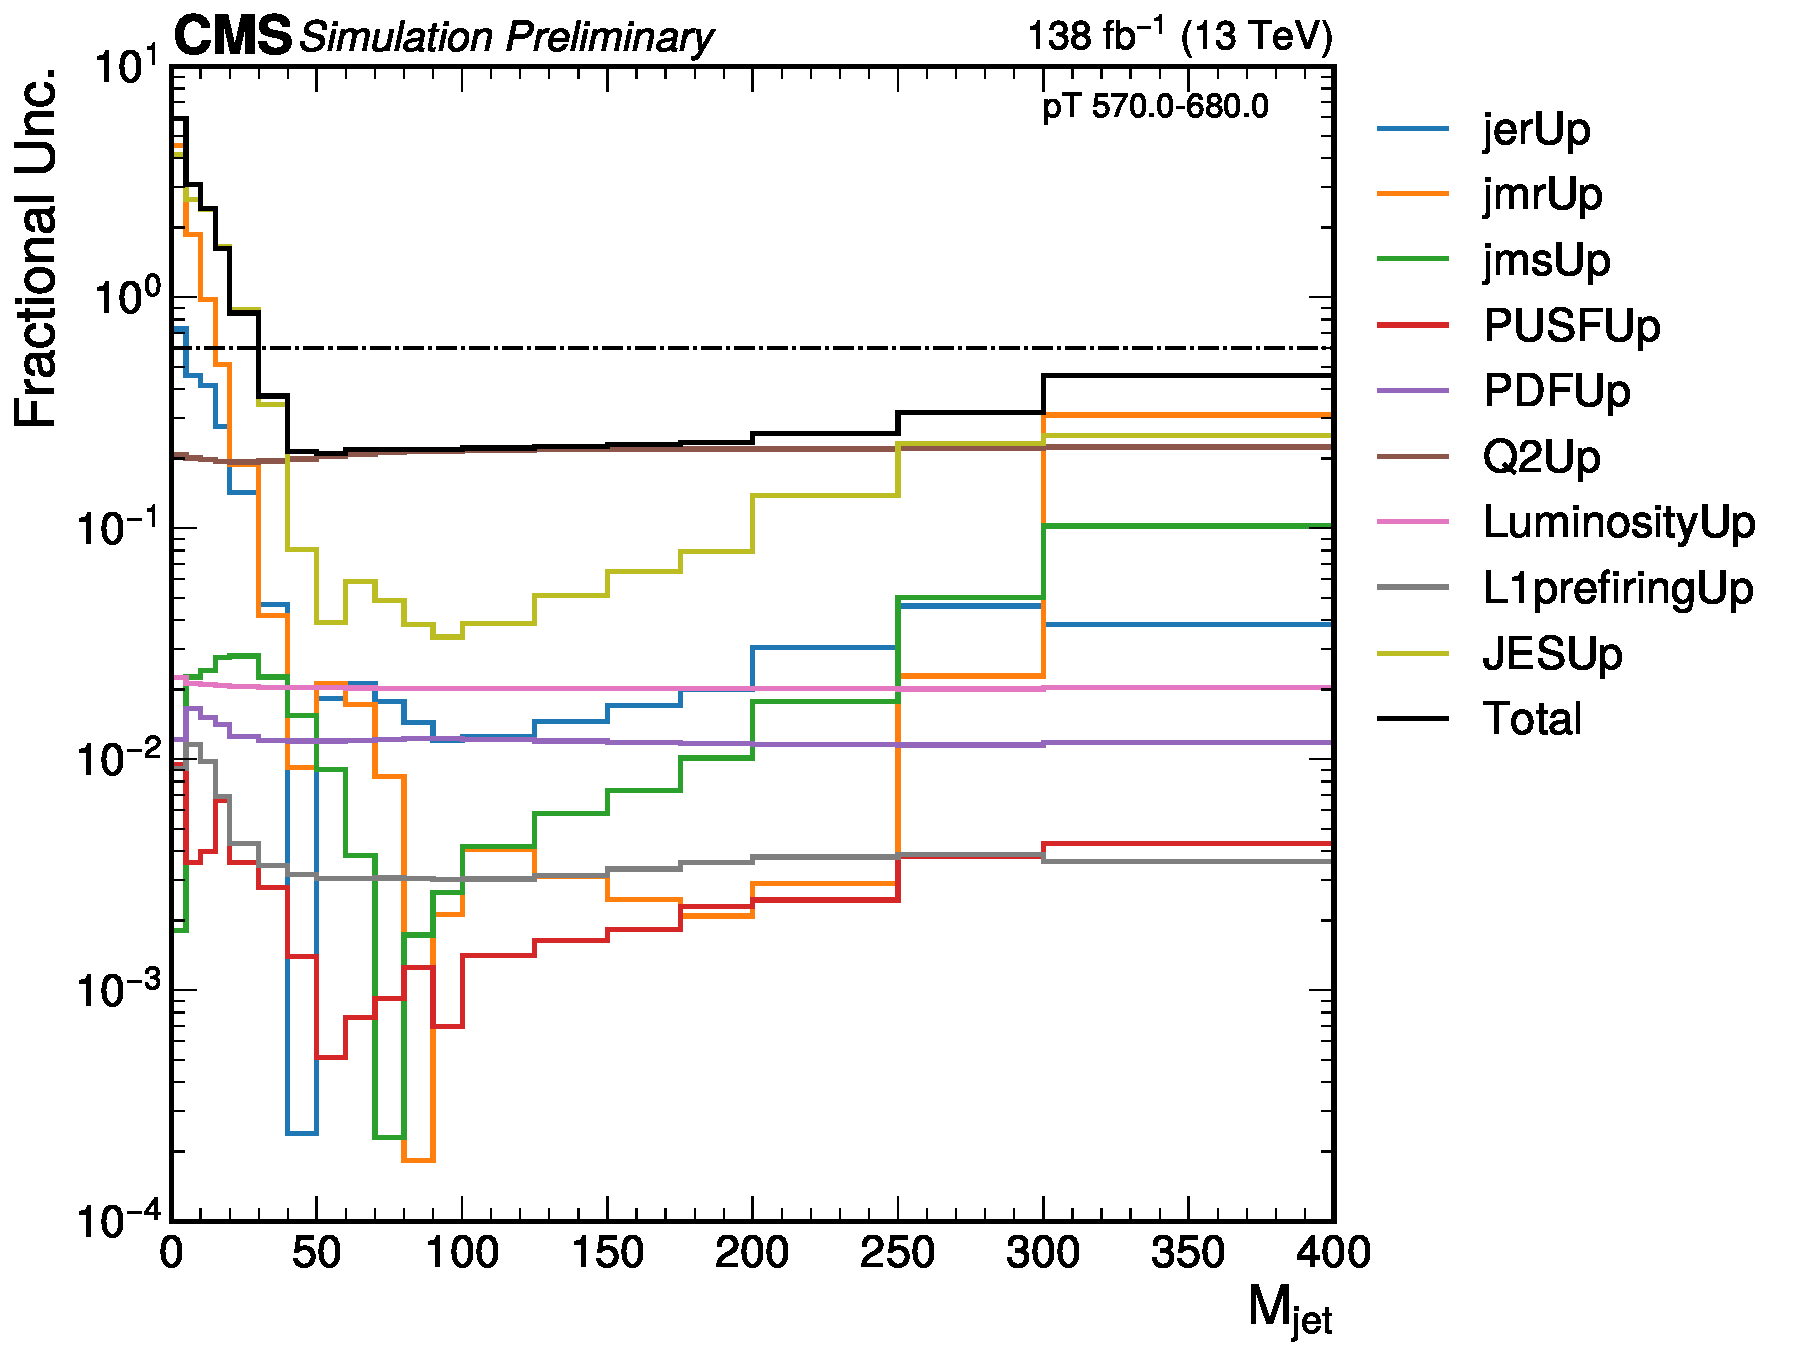
\includegraphics[width=0.45\textwidth]{figures/multijet/dijet/fracUnc_ungroomed_3.pdf}
\end{subfigure}
  \begin{subfigure}
    \centering
    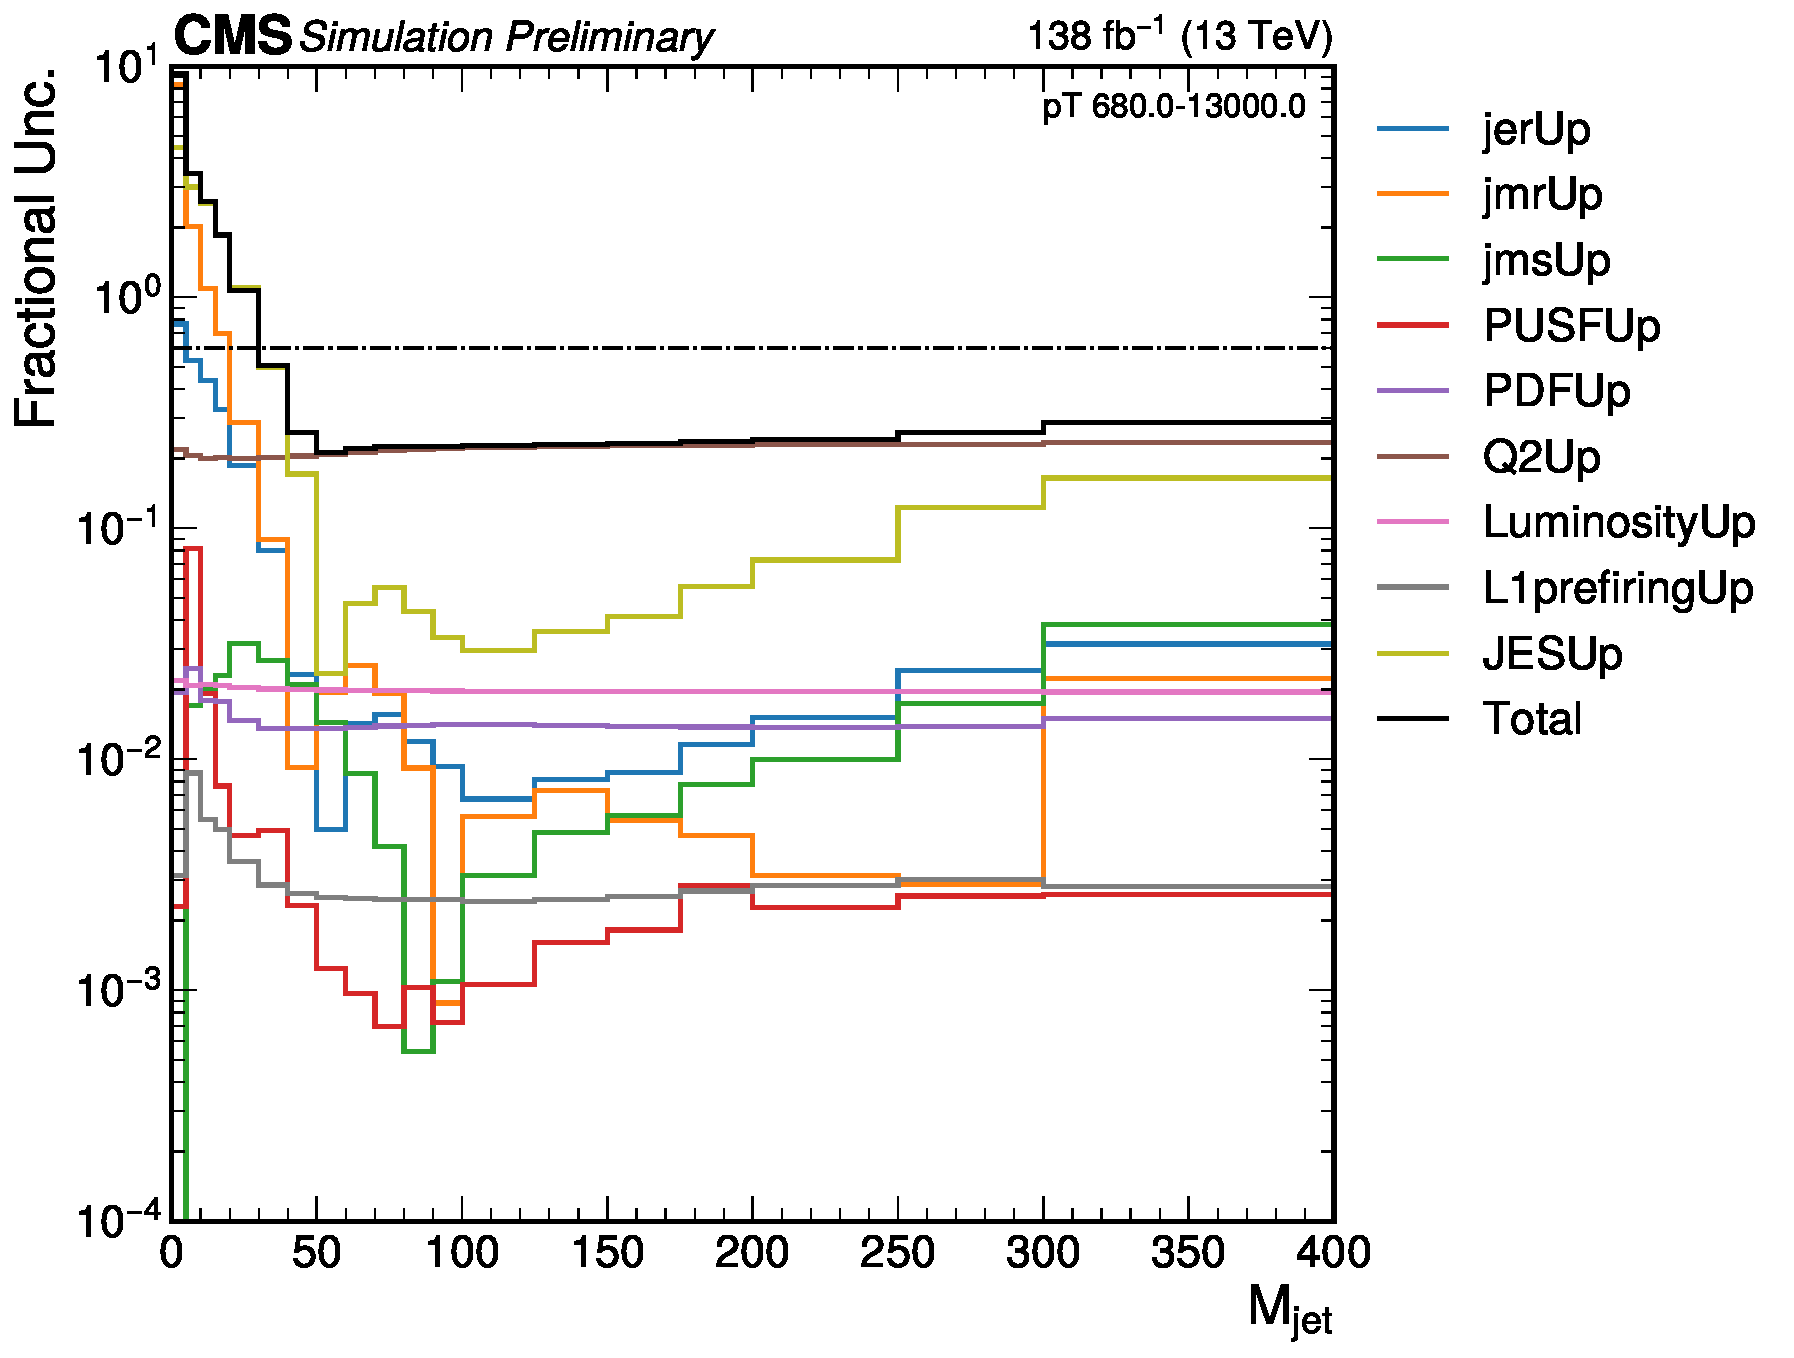
\includegraphics[width=0.45\textwidth]{figures/multijet/dijet/fracUnc_ungroomed_4.pdf}
\end{subfigure}
  \caption{Uncertainties per bin before unfolding in the ungroomed dijet channel.}
  \label{fig:dijetunc_ungroomed}
  \end{figure}
\begin{figure}[ht!]
  \centering
  \begin{subfigure}
    \centering
    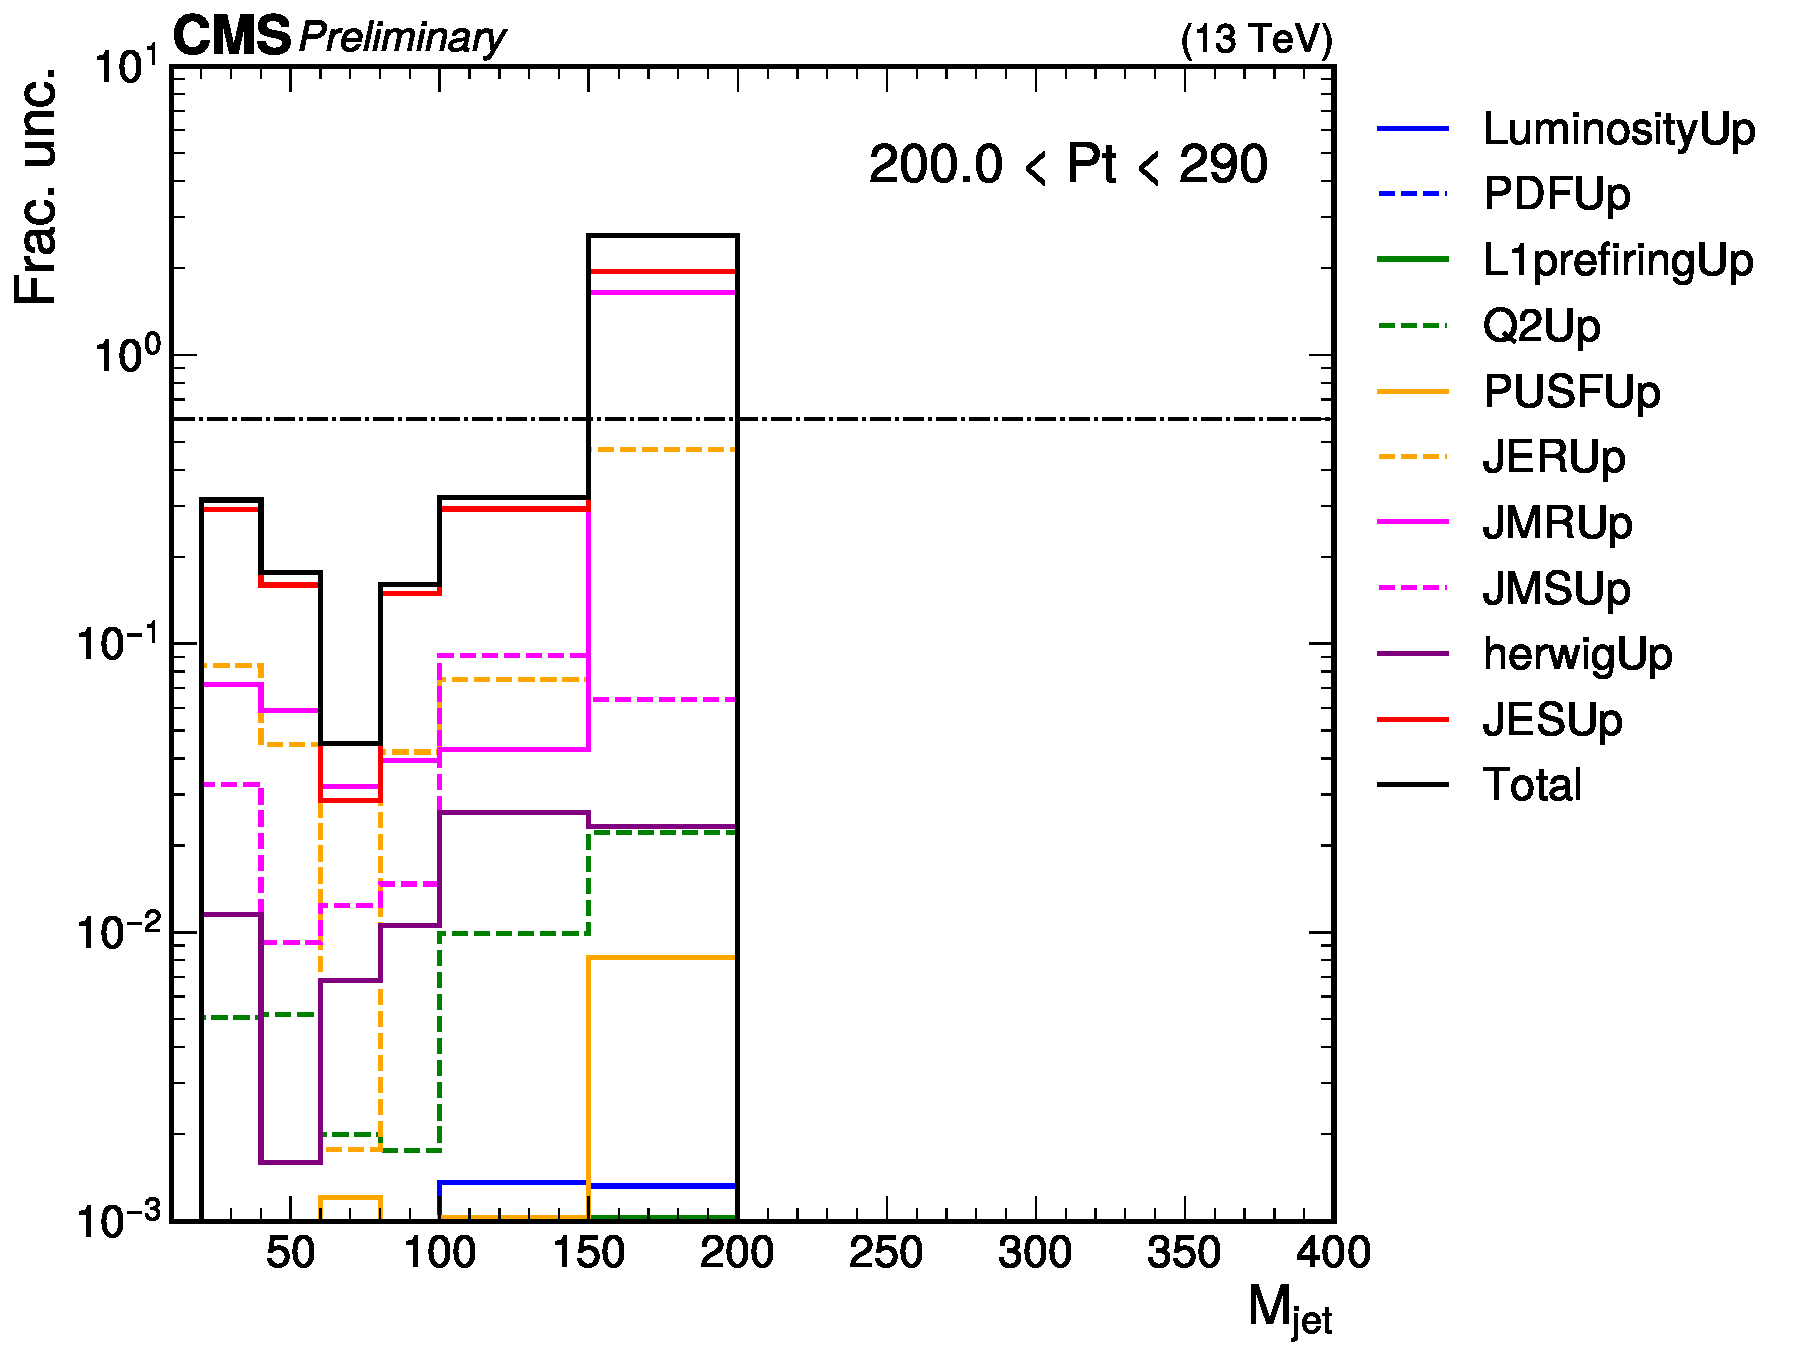
\includegraphics[width=0.45\textwidth]{figures/multijet/unfolding/dijet/unfolded_fracUnc_ungroomed_0.pdf}
\end{subfigure}
  \begin{subfigure}
    \centering
    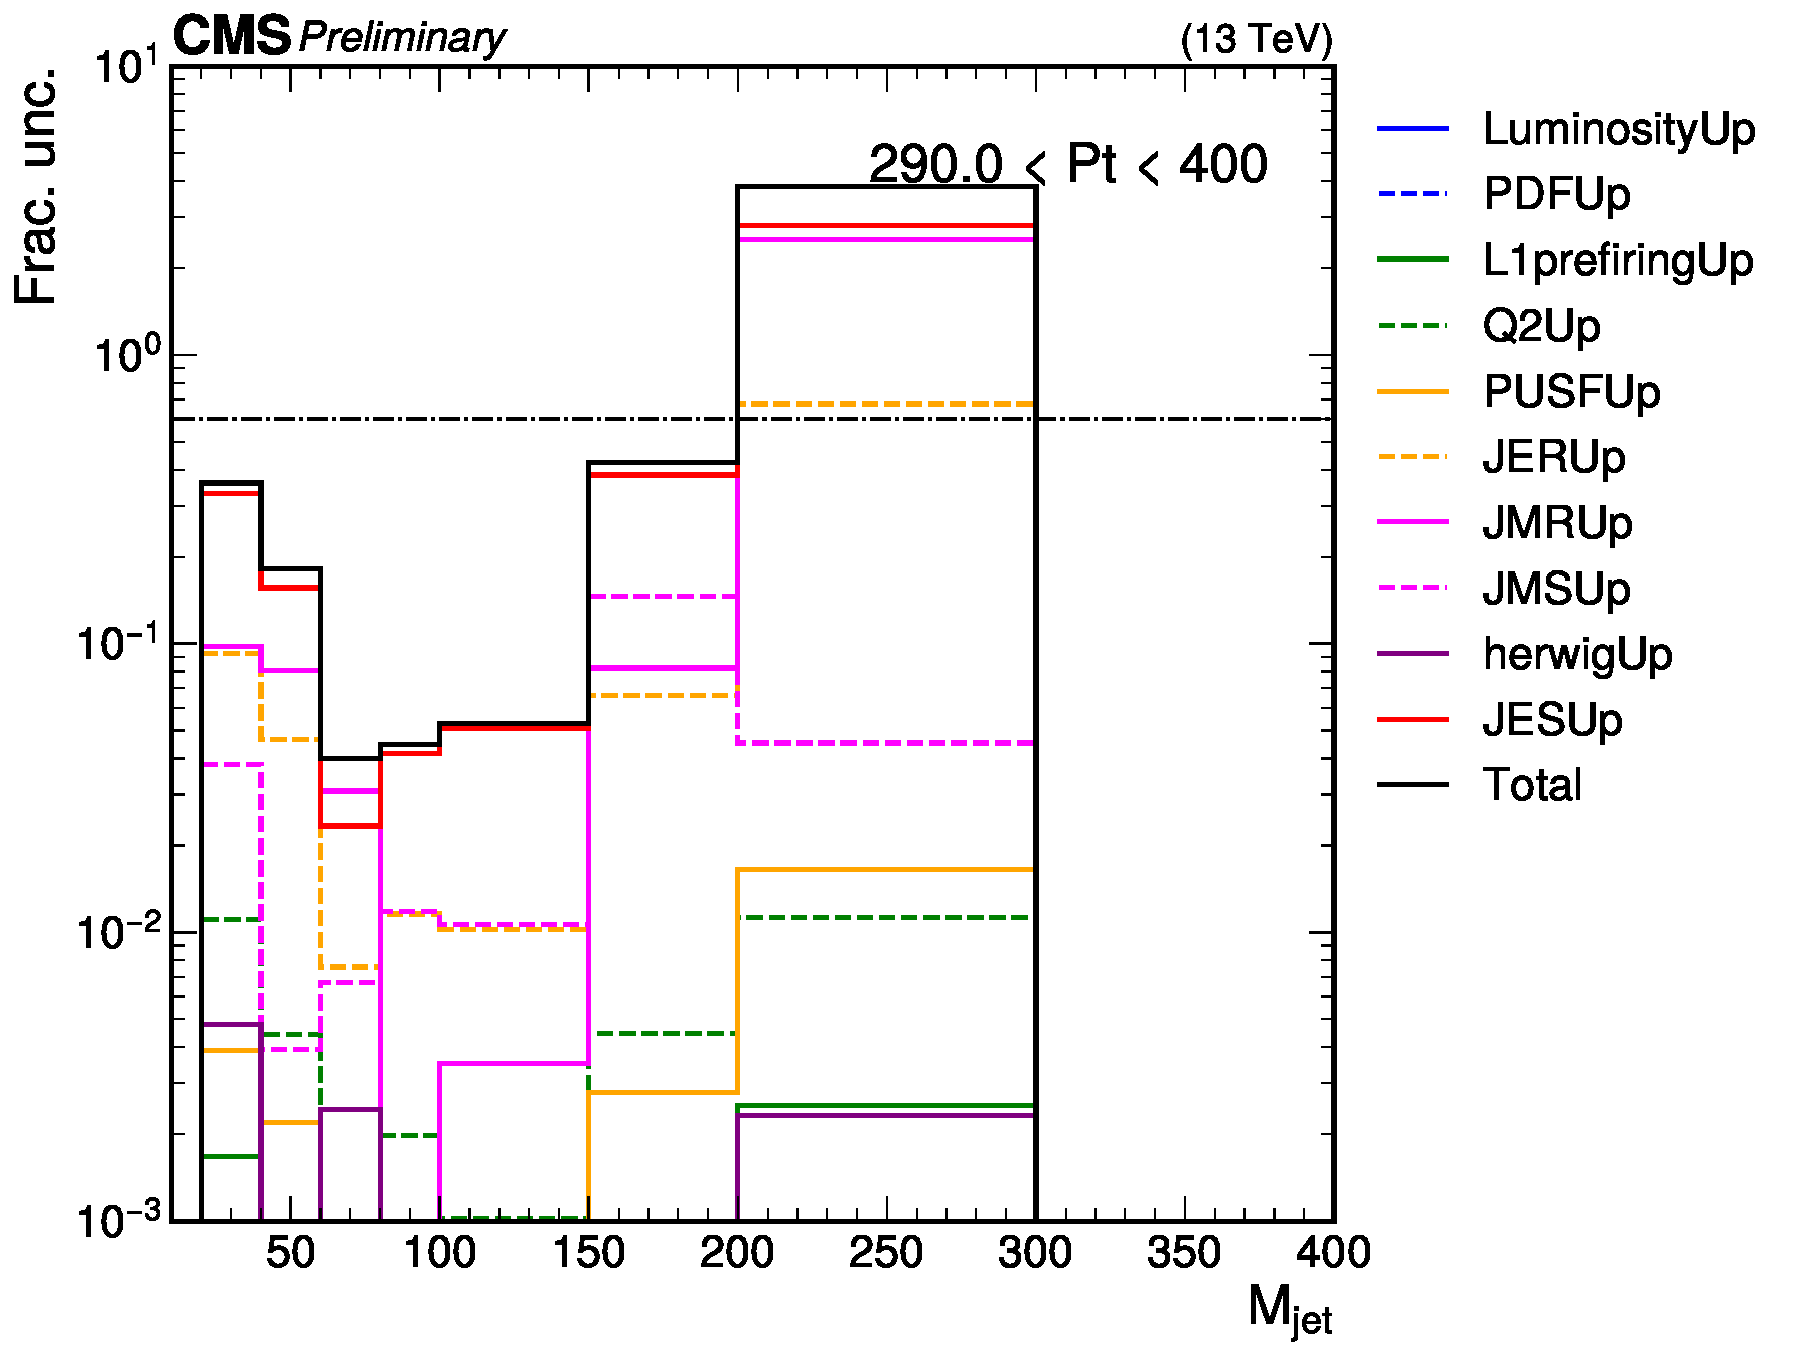
\includegraphics[width=0.45\textwidth]{figures/multijet/unfolding/dijet/unfolded_fracUnc_ungroomed_1.pdf}
\end{subfigure}
  \begin{subfigure}
    \centering
    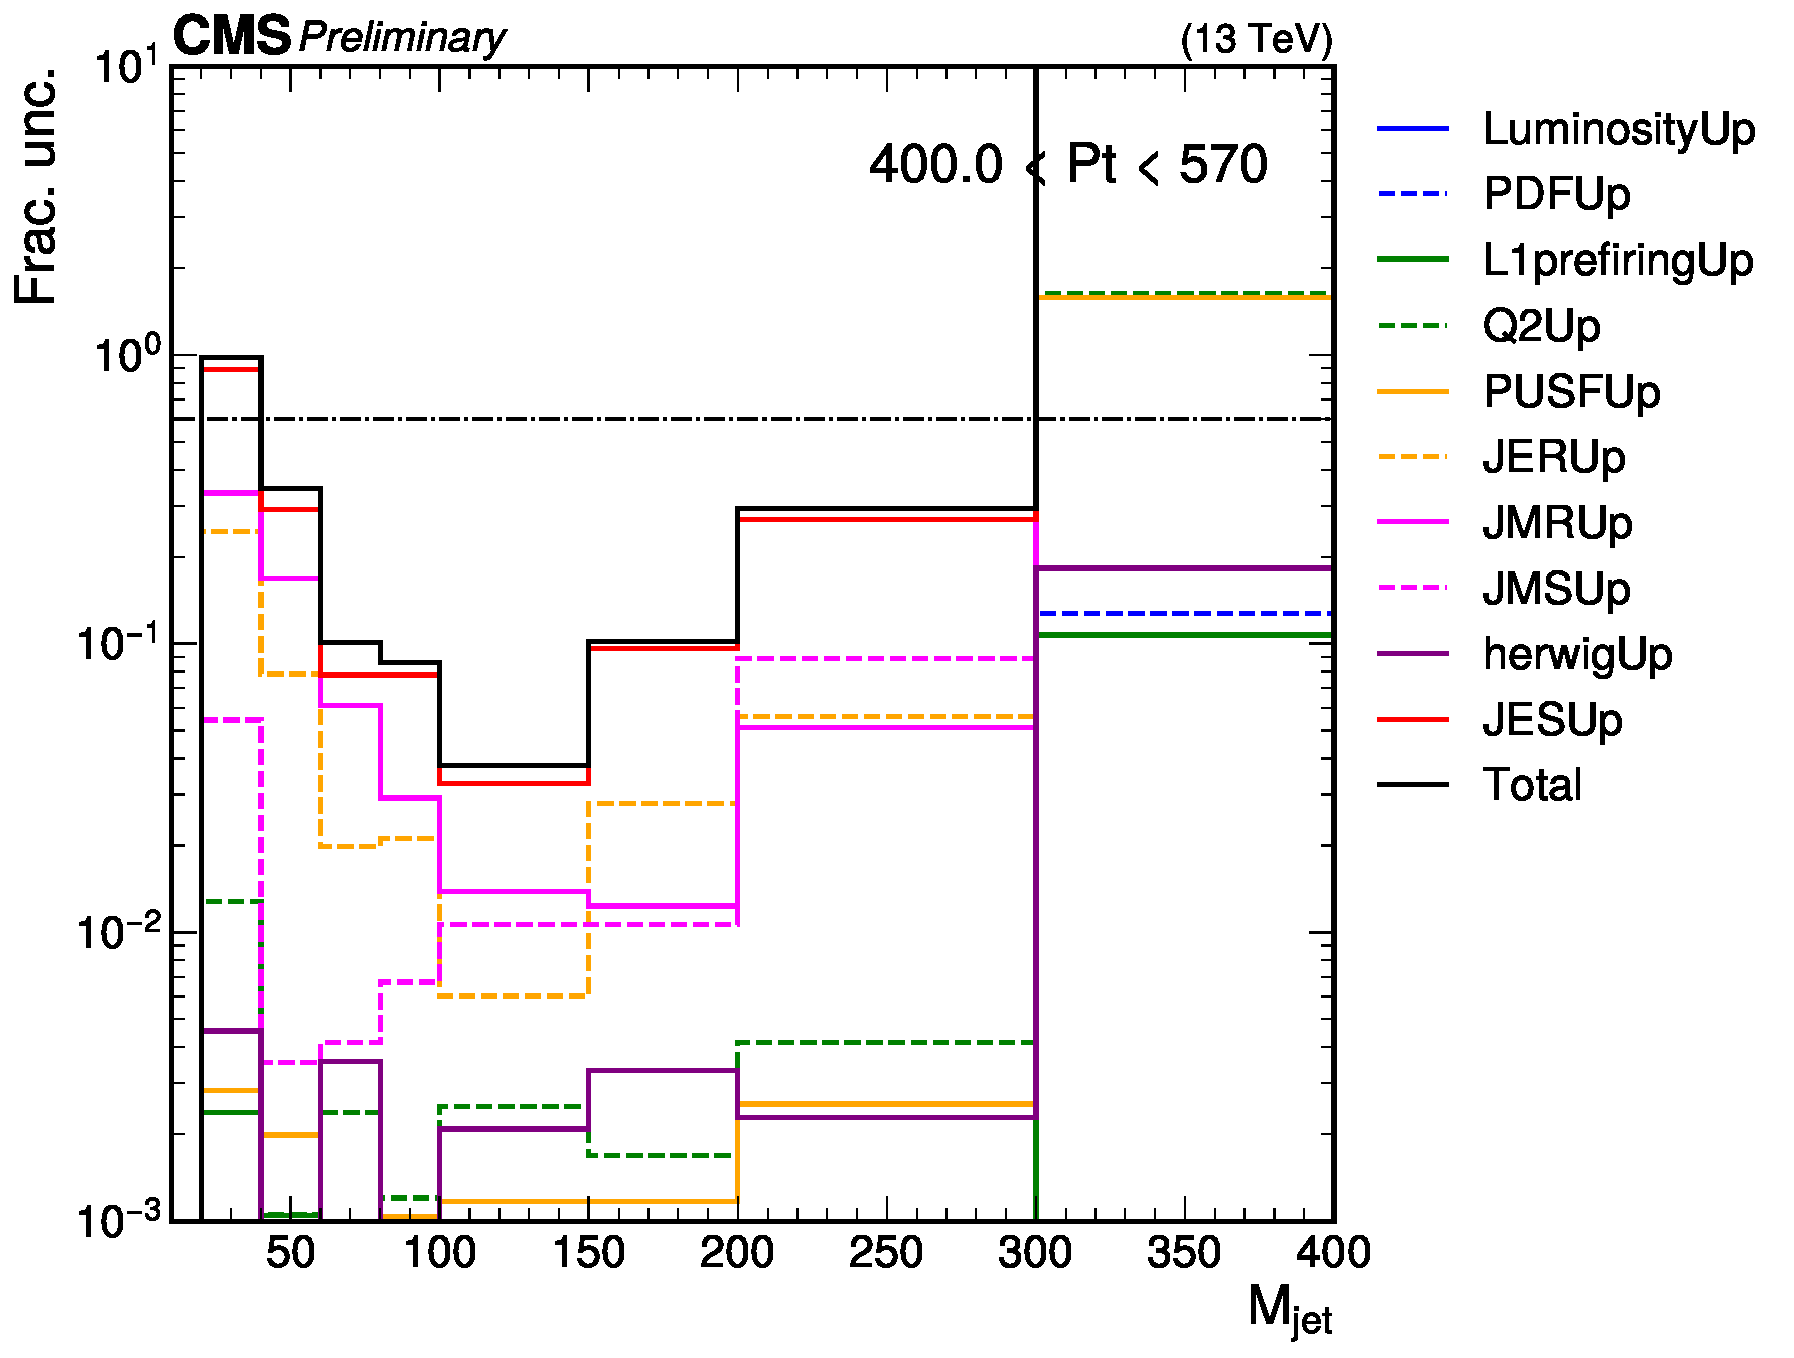
\includegraphics[width=0.45\textwidth]{figures/multijet/unfolding/dijet/unfolded_fracUnc_ungroomed_2.pdf}
\end{subfigure}
\begin{subfigure}
    \centering
    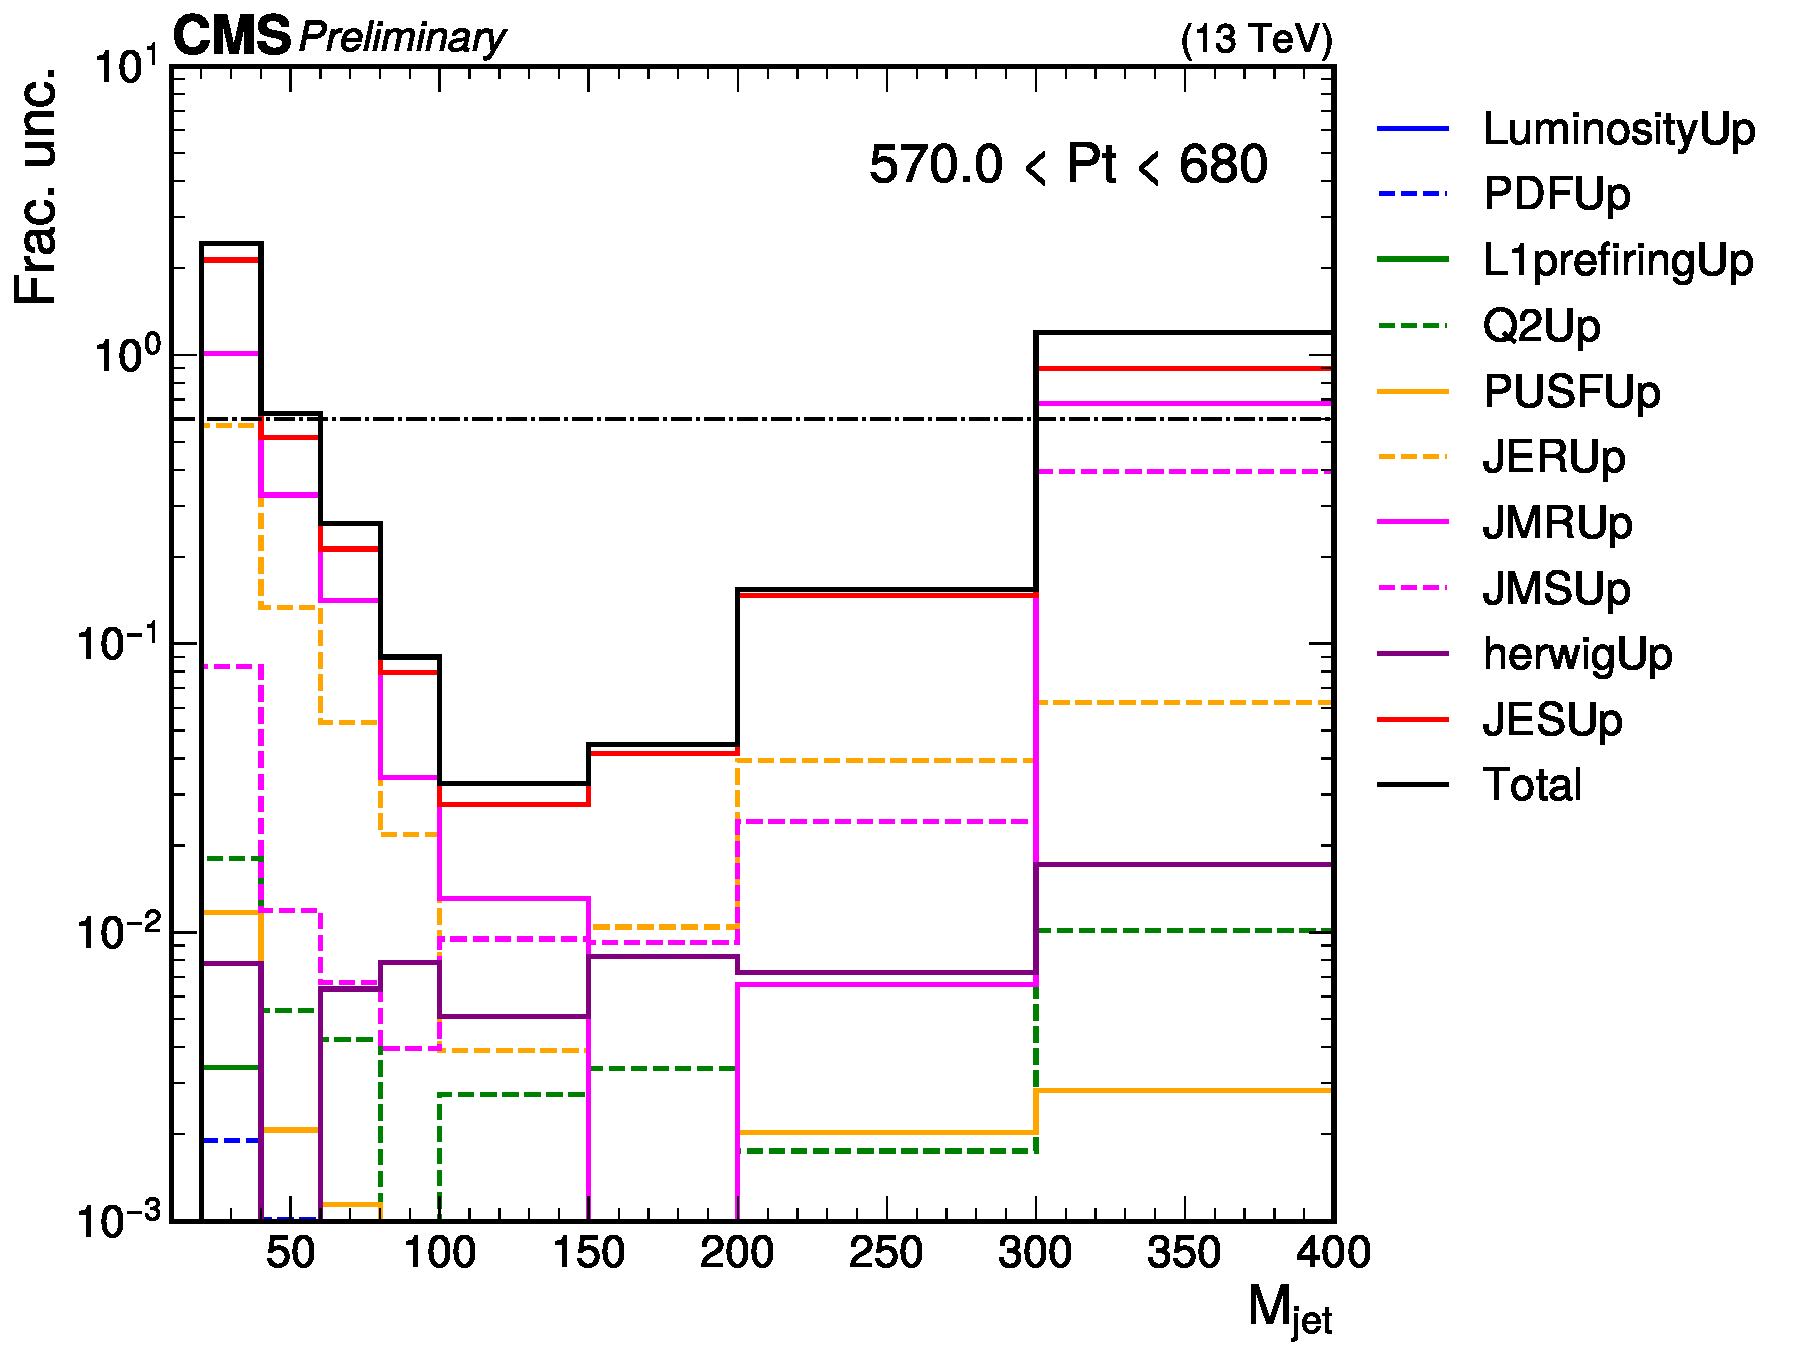
\includegraphics[width=0.45\textwidth]{figures/multijet/unfolding/dijet/unfolded_fracUnc_ungroomed_3.pdf}
\end{subfigure}
  \begin{subfigure}
    \centering
    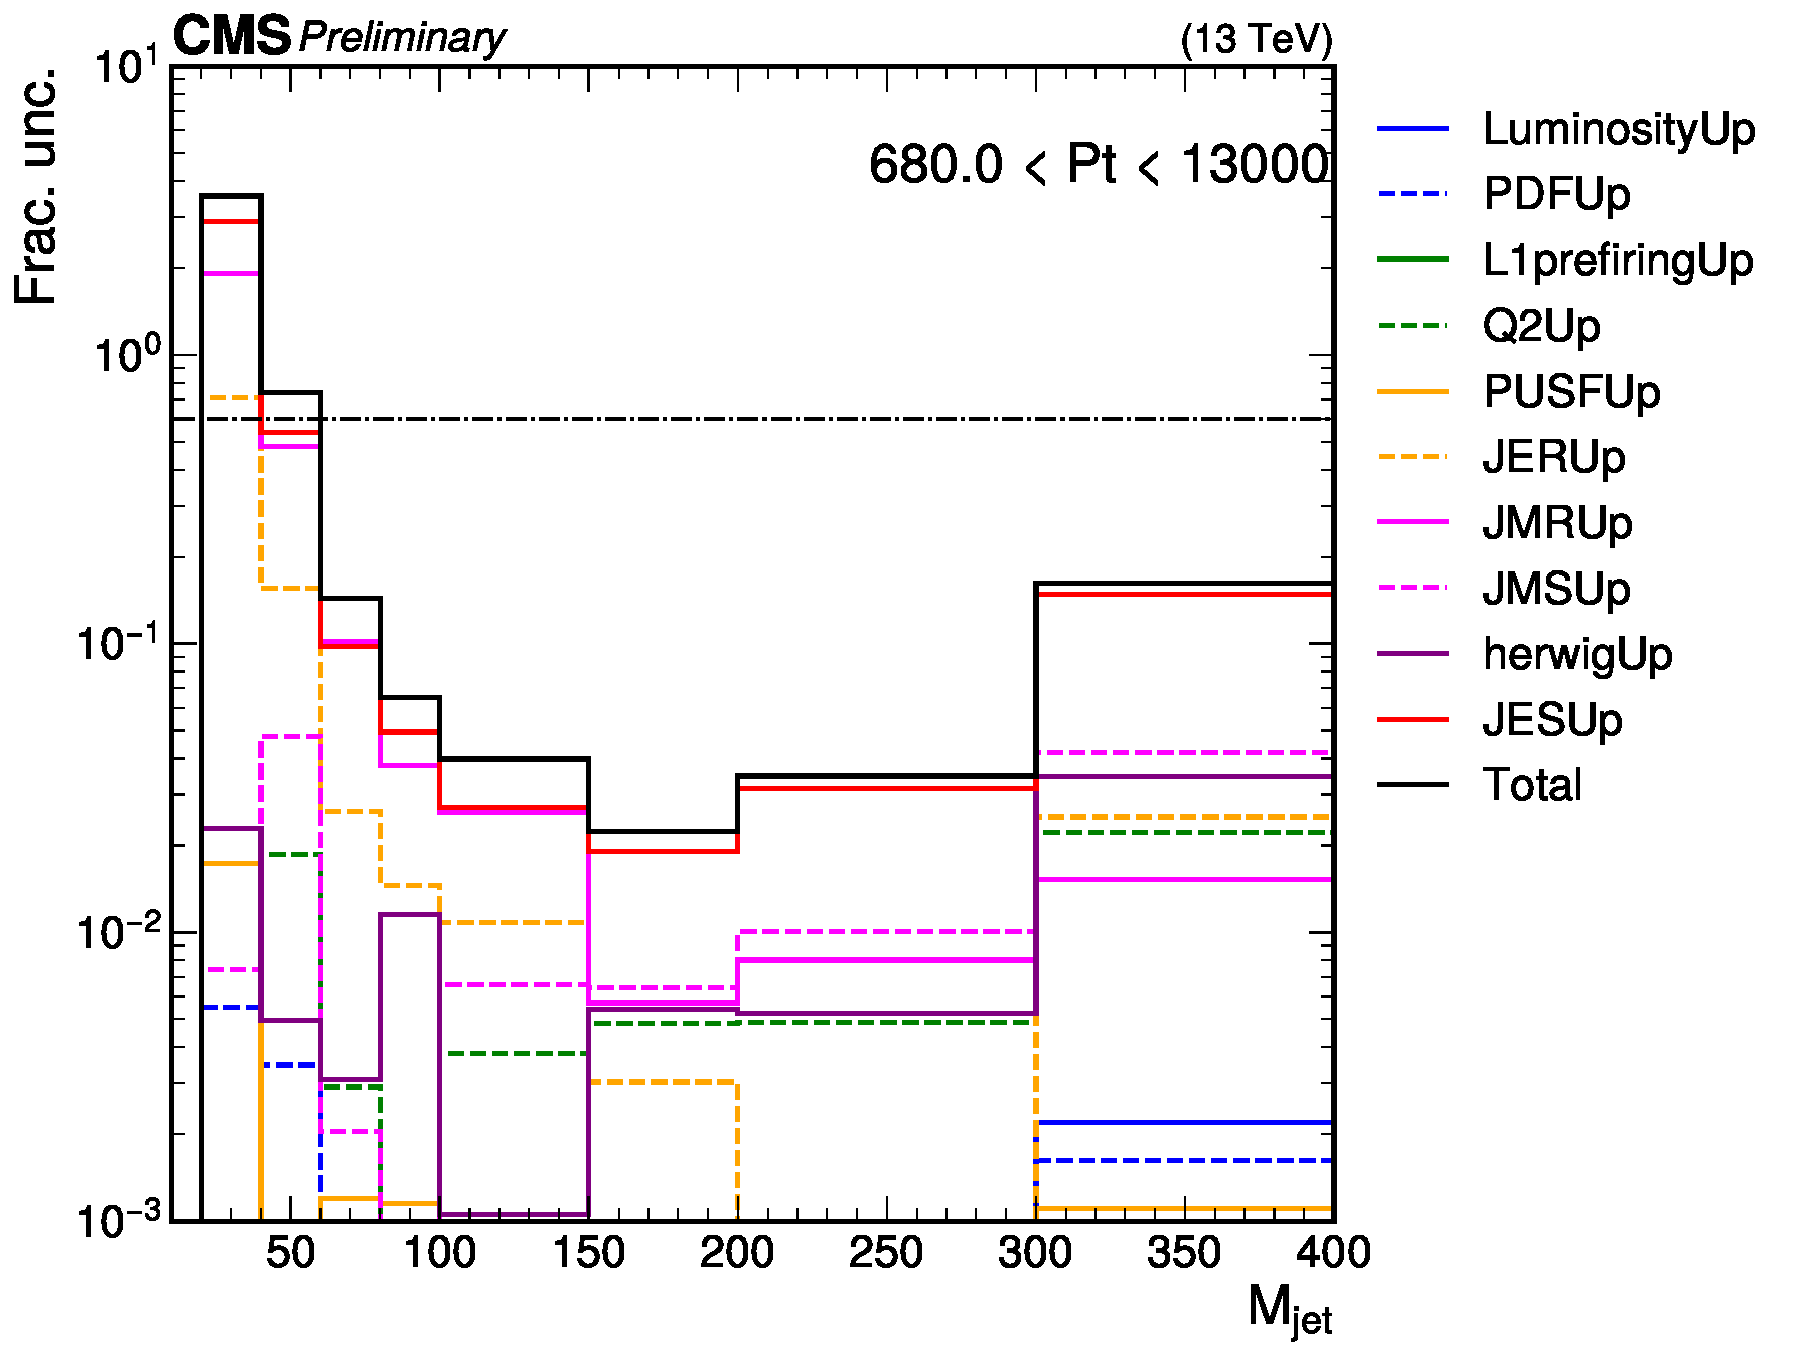
\includegraphics[width=0.45\textwidth]{figures/multijet/unfolding/dijet/unfolded_fracUnc_ungroomed_4.pdf}
\end{subfigure}
  \caption{Uncertainties per bin and after unfolding in the ungroomed dijet channel.}
  \label{fig:dijetunc_ungroomed_postunfold}
\end{figure}
\begin{figure}[ht!]
  \centering
  \begin{subfigure}
    \centering
    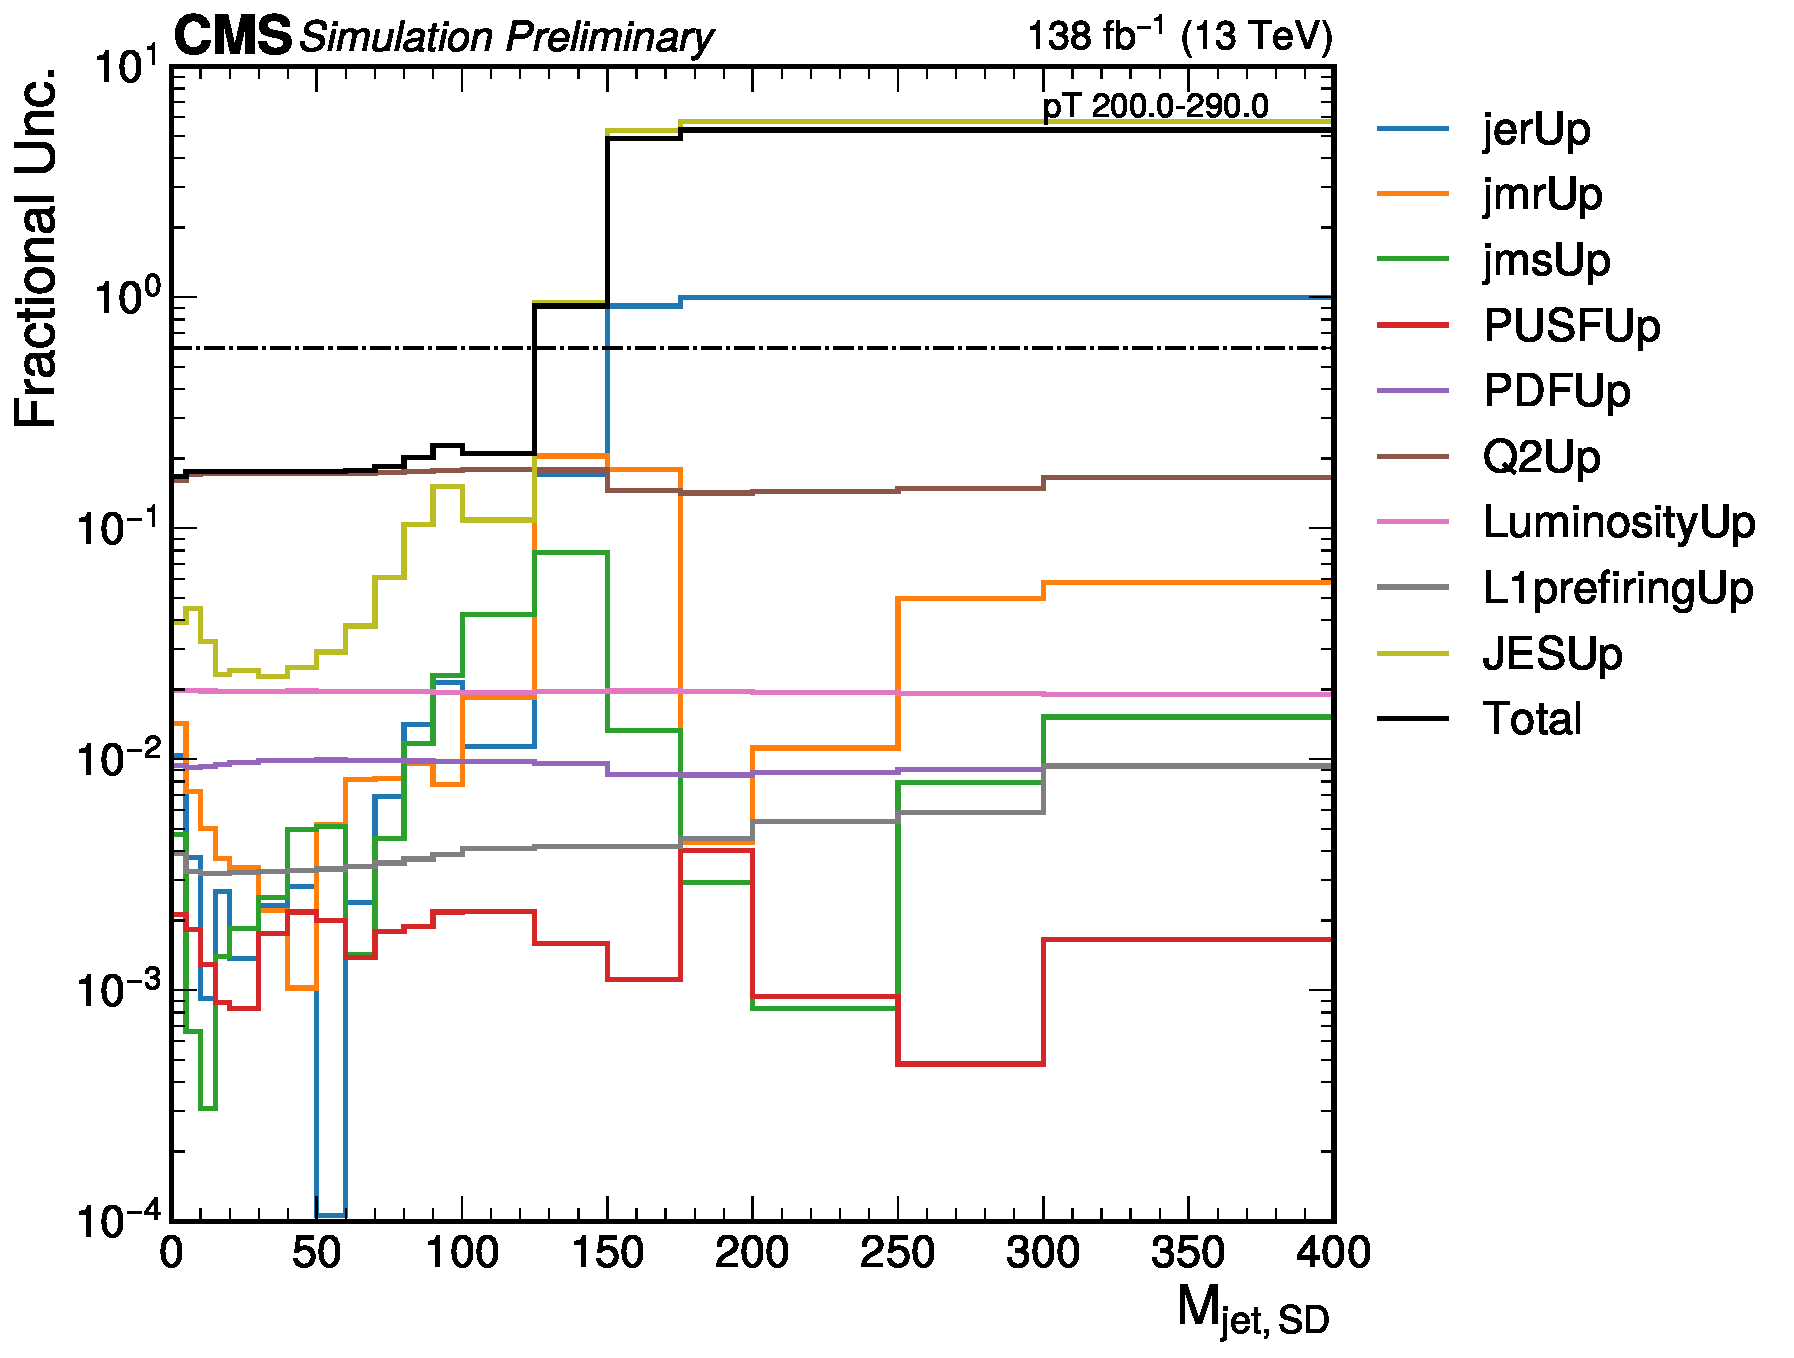
\includegraphics[width=0.45\textwidth]{figures/multijet/dijet/fracUnc_groomed_0.pdf}
\end{subfigure} 
  \begin{subfigure}
    \centering
    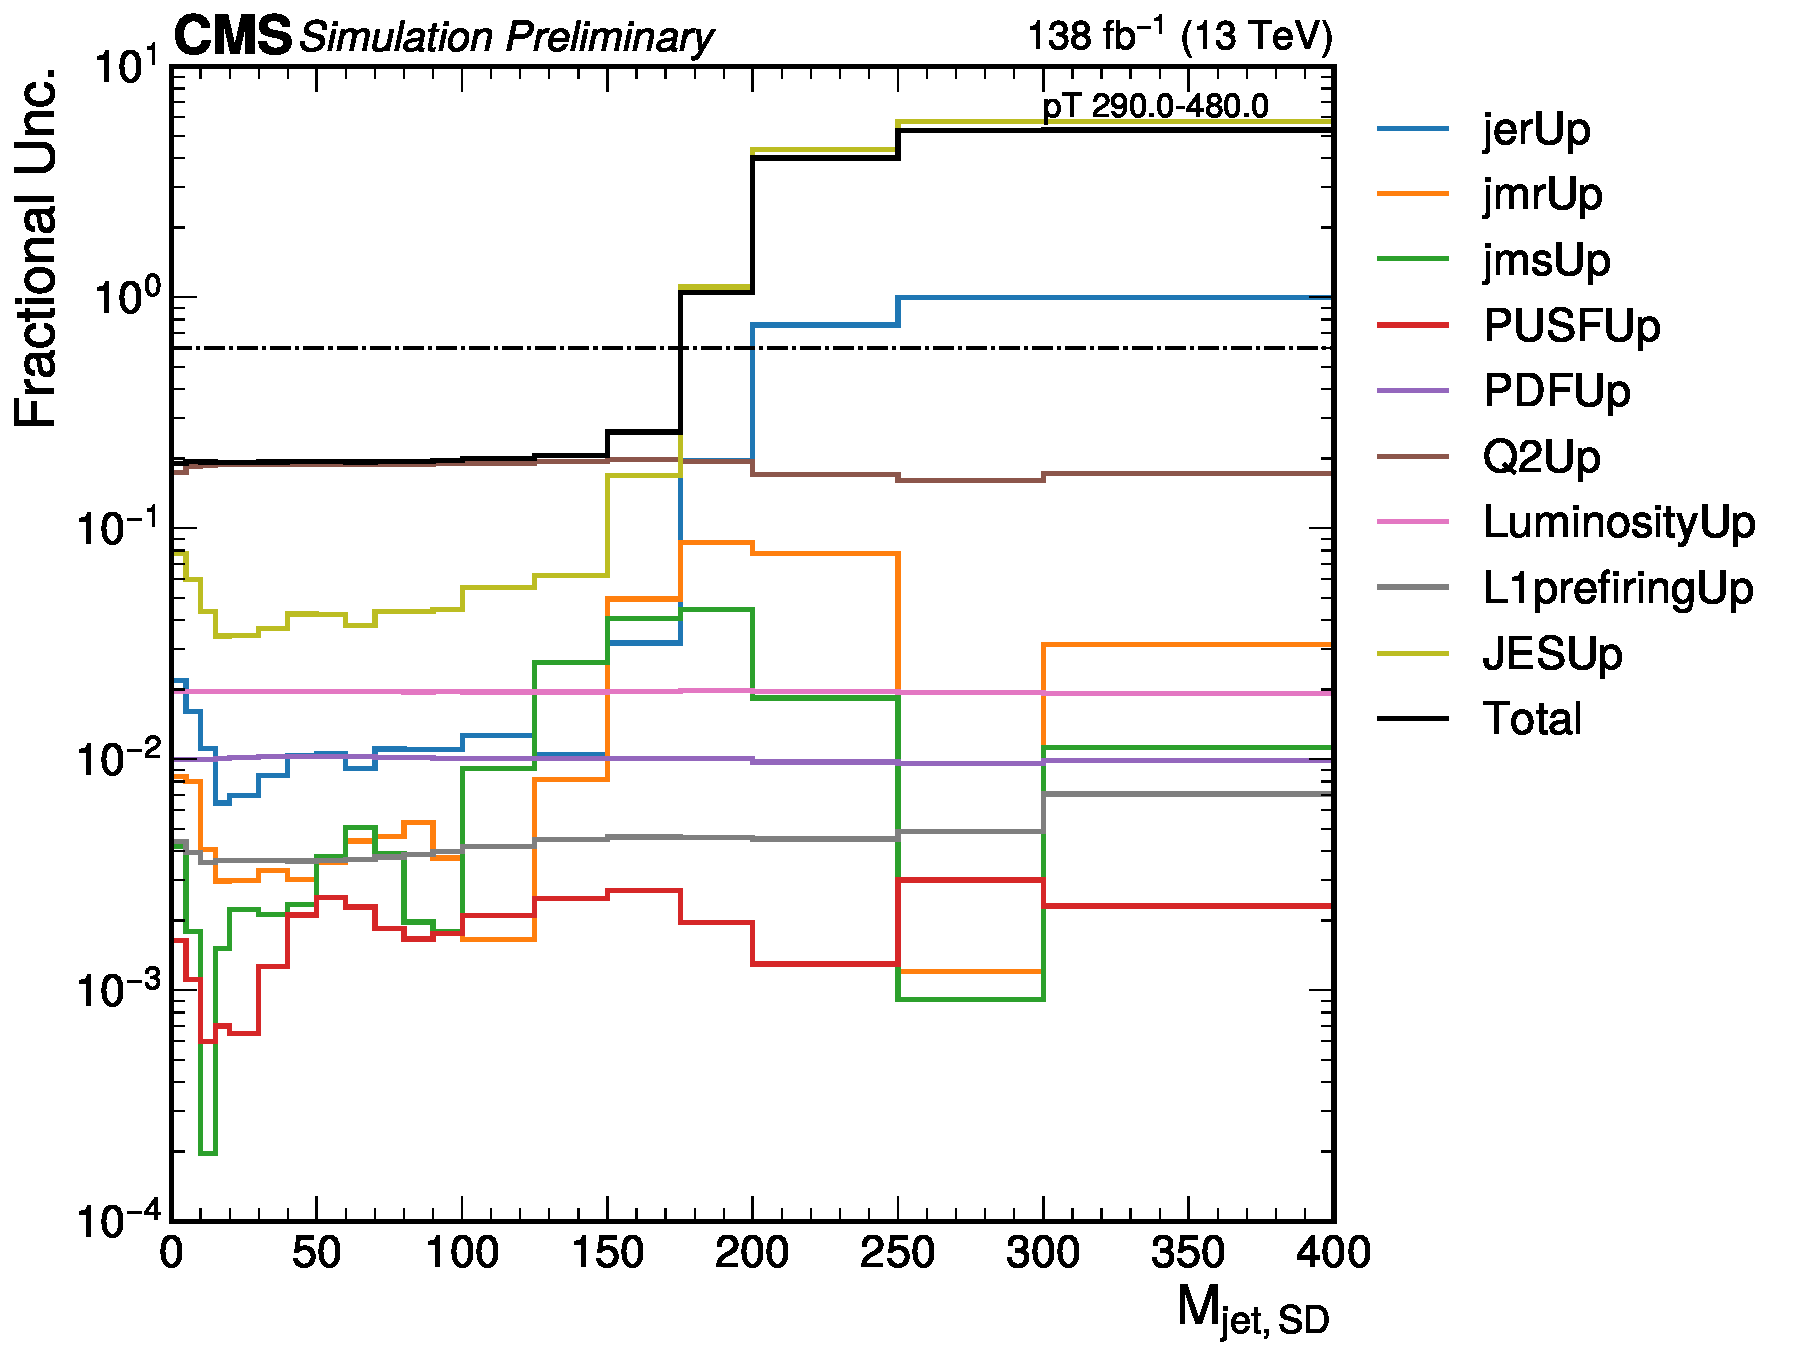
\includegraphics[width=0.45\textwidth]{figures/multijet/dijet/fracUnc_groomed_1.pdf}
\end{subfigure}
  \begin{subfigure}
    \centering
    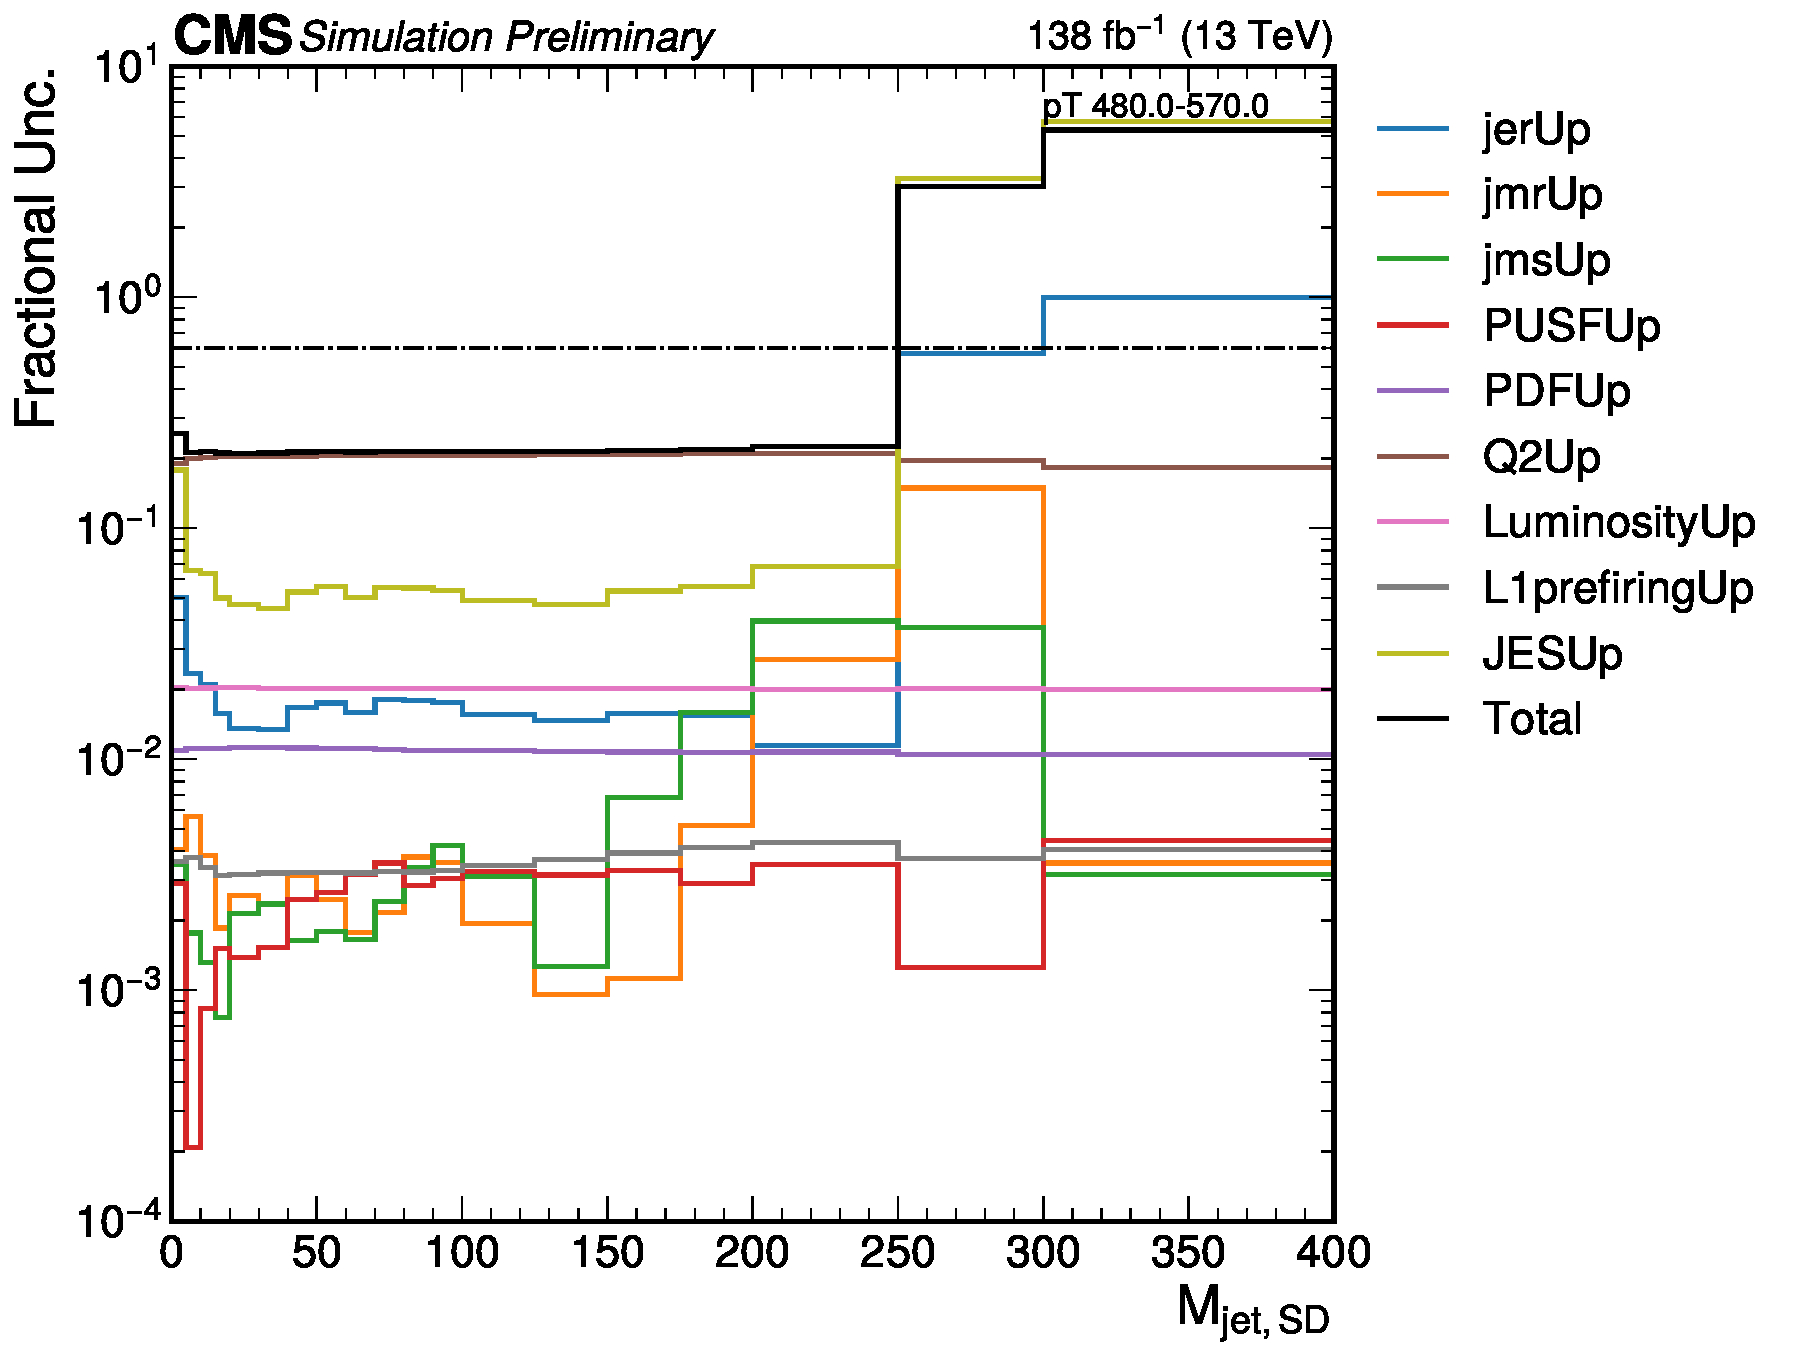
\includegraphics[width=0.45\textwidth]{figures/multijet/dijet/fracUnc_groomed_2.pdf}
\end{subfigure}
  \begin{subfigure}
    \centering
    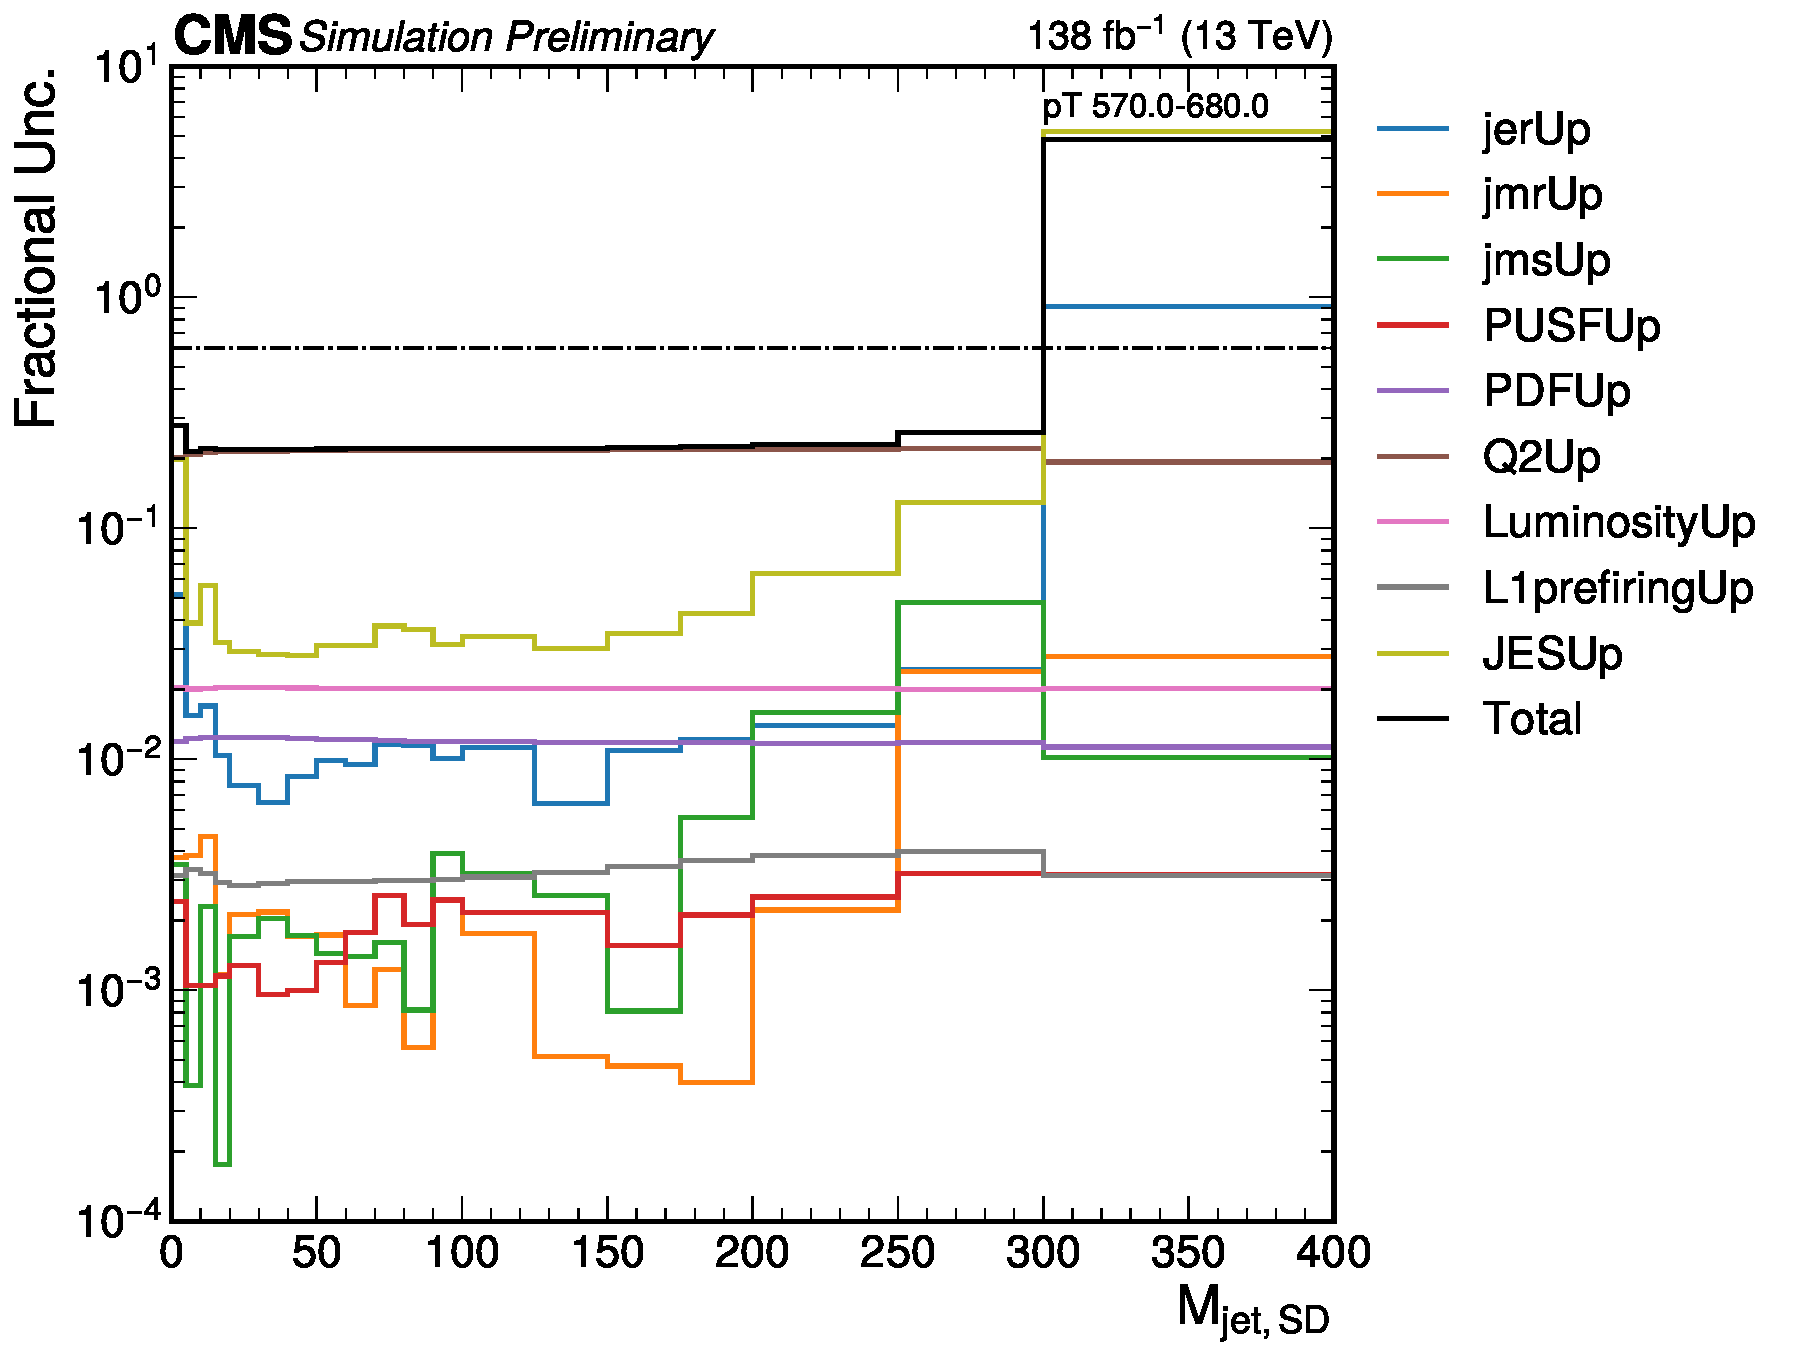
\includegraphics[width=0.45\textwidth]{figures/multijet/dijet/fracUnc_groomed_3.pdf}
\end{subfigure}
  \begin{subfigure}
    \centering
    \includegraphics[width=0.45\textwidth]{figures/multijet/dijet/fracUnc_groomed_4.pdf}
\end{subfigure}
  \caption{Uncertainties per bin before unfolding in the groomed dijet channel.}
  \label{fig:dijetunc_groomed}
  \end{figure}
\begin{figure}[ht!]
  \centering
  \begin{subfigure}
    \centering
    \includegraphics[width=0.45\textwidth]{figures/multijet/unfolding/dijet/unfolded_fracUnc_groomed_0.png}
\end{subfigure}
  \begin{subfigure}
    \centering
    \includegraphics[width=0.45\textwidth]{figures/multijet/unfolding/dijet/unfolded_fracUnc_groomed_1.png}
\end{subfigure}
  \begin{subfigure}
    \centering
    \includegraphics[width=0.45\textwidth]{figures/multijet/unfolding/dijet/unfolded_fracUnc_groomed_2.png}
\end{subfigure}
\begin{subfigure}
    \centering
    \includegraphics[width=0.45\textwidth]{figures/multijet/unfolding/dijet/unfolded_fracUnc_groomed_3.png}
\end{subfigure}
  \begin{subfigure}
    \centering
    \includegraphics[width=0.45\textwidth]{figures/multijet/unfolding/dijet/unfolded_fracUnc_groomed_4.png}
\end{subfigure}
  \caption{Uncertainties per bin and after unfolding in the groomed dijet channel.}
  \label{fig:dijetunc_groomed_postunfold}
\end{figure}
\begin{figure}[ht!]
  \centering
  \begin{subfigure}
    \centering
    \includegraphics[width=0.45\textwidth]{figures/multijet/trijet/fracUnc_ungroomed_0.pdf}
\end{subfigure} 
  \begin{subfigure}
    \centering
    \includegraphics[width=0.45\textwidth]{figures/multijet/trijet/fracUnc_ungroomed_1.pdf}
\end{subfigure}
  \begin{subfigure}
    \centering
    \includegraphics[width=0.45\textwidth]{figures/multijet/trijet/fracUnc_ungroomed_2.pdf}
\end{subfigure}
  \begin{subfigure}
    \centering
    \includegraphics[width=0.45\textwidth]{figures/multijet/trijet/fracUnc_ungroomed_3.pdf}
\end{subfigure}
  \caption{Uncertainties per bin before unfolding in the ungroomed trijet channel.}
  \label{fig:trijetunc_ungroomed}
  \end{figure}
\begin{figure}[ht!]
  \centering
  \begin{subfigure}
    \centering
    \includegraphics[width=0.45\textwidth]{figures/multijet/unfolding/trijet/unfolded_fracUnc_ungroomed_0.pdf}
\end{subfigure}
  \begin{subfigure}
    \centering
    \includegraphics[width=0.45\textwidth]{figures/multijet/unfolding/trijet/unfolded_fracUnc_ungroomed_1.pdf}
\end{subfigure}
  \begin{subfigure}
    \centering
    \includegraphics[width=0.45\textwidth]{figures/multijet/unfolding/trijet/unfolded_fracUnc_ungroomed_2.pdf}
\end{subfigure}
\begin{subfigure}
    \centering
    \includegraphics[width=0.45\textwidth]{figures/multijet/unfolding/trijet/unfolded_fracUnc_ungroomed_3.pdf}
\end{subfigure}
  \caption{Uncertainties per bin and after unfolding in the ungroomed trijet channel.}
  \label{fig:trijetunc_ungroomed_postunfold}
\end{figure}
\begin{figure}[ht!]
  \centering
  \begin{subfigure}
    \centering
    \includegraphics[width=0.45\textwidth]{figures/multijet/trijet/fracUnc_groomed_0.pdf}
\end{subfigure} 
  \begin{subfigure}
    \centering
    \includegraphics[width=0.45\textwidth]{figures/multijet/trijet/fracUnc_groomed_1.pdf}
\end{subfigure}
  \begin{subfigure}
    \centering
    \includegraphics[width=0.45\textwidth]{figures/multijet/trijet/fracUnc_groomed_2.pdf}
\end{subfigure}
  \begin{subfigure}
    \centering
    \includegraphics[width=0.45\textwidth]{figures/multijet/trijet/fracUnc_groomed_3.pdf}
\end{subfigure}
  \caption{Uncertainties per bin before unfolding in the groomed trijet channel.}
  \label{fig:trijetunc_groomed}
  \end{figure}
\begin{figure}[ht!]
  \centering
  \begin{subfigure}
    \centering
    \includegraphics[width=0.45\textwidth]{figures/multijet/unfolding/trijet/unfolded_fracUnc_groomed_0.png}
\end{subfigure}
  \begin{subfigure}
    \centering
    \includegraphics[width=0.45\textwidth]{figures/multijet/unfolding/trijet/unfolded_fracUnc_groomed_1.png}
\end{subfigure}
  \begin{subfigure}
    \centering
    \includegraphics[width=0.45\textwidth]{figures/multijet/unfolding/trijet/unfolded_fracUnc_groomed_2.png}
\end{subfigure}
\begin{subfigure}
    \centering
    \includegraphics[width=0.45\textwidth]{figures/multijet/unfolding/trijet/unfolded_fracUnc_groomed_3.png}
\end{subfigure}
  \caption{Uncertainties per bin and after unfolding in the groomed trijet channel.}
  \label{fig:trijetunc_groomed_postunfold}
\end{figure}
